% !TEX root = ../partial-sdm.tex

\chapter{Results (vi): Supervised classification application}

Supervised classification problem consists of categorizing data into groups after seeing some samples from each group. First, it is presented pieces of data with their categories. The algorithm learns from these data, which is known as the learning phase. Then, new pieces of data are presented and the algorithm must classify them into the already known groups. It is named ``supervised'' because  the algorithm will not create the groups itself. It will learn the groups during the learning phase, in which the groups have already been defined and the pieces of data have already been classified into them.

Although this problem has already been studied (REF), our intention here is to show that a pure SDM may also be used to classify data. \citet{fan1997genetic} has used SDM to solve a classification problem, recognizing handwriting letters from images, but he used a mix of genetic algorithm with SDM, which is very different from the original SDM described by \cite{Kanerva1988}. Even though his algorithm has classified properly, we were intrigued whether a pure SDM would also classify successfully.

Hence, we have developed a supervised classification algorithm based on a pure SDM as our main memory. Our goal was to classify noisy images into their respective letters (case sensitive) and numbers. For some examples, see Figure \ref{fig-classification-examples}.

\begin{figure}[!htb]
\centering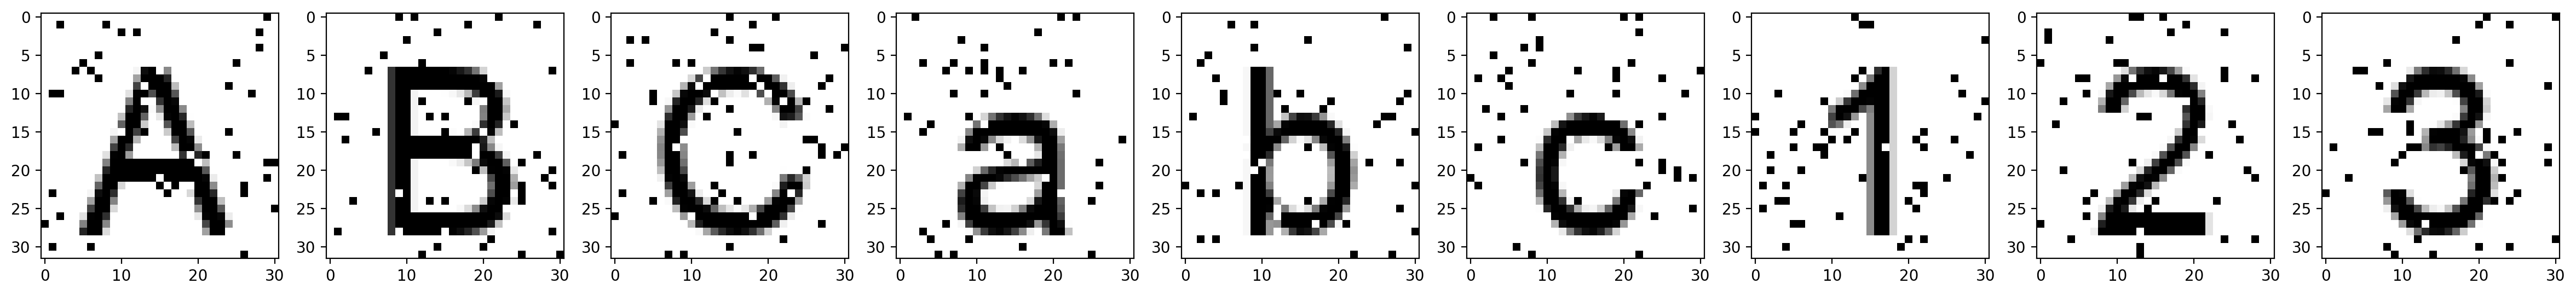
\includegraphics[width=\textwidth]{./images02/classification/example.png}
\caption{Examples of noisy images with uppercase letters, lowercase letters, and numbers.
\label{fig-classification-examples}}
\end{figure}

The images had 31 pixels of width and 32 pixels of height, totaling 992 pixels per image. Each image was mapped into a 1,000-bit bitstring in which the bits were set according to the color of each pixel of the image. So, white pixels were equal to bit 0, and black pixels to bit 1. The eight remaining bits were all set to zero. This was a bijective mapping (or one-to-one mapping), i.e., there was only one bitstring for each image, and there was only one image for each bitstring.

% TODO Add image showing the association between pixels and bits.

A total of 62 classification groups have been trained in the SDM. For each of them, it was generated a random bitstring. Thus, the groups' bitstrings were orthogonal between any two of them. There is one image for each of the 62 groups in Figure \ref{fig-classification-groups}. Notice that the SDM has never seen a single image with no noise.

\begin{figure}[!htb]
\centering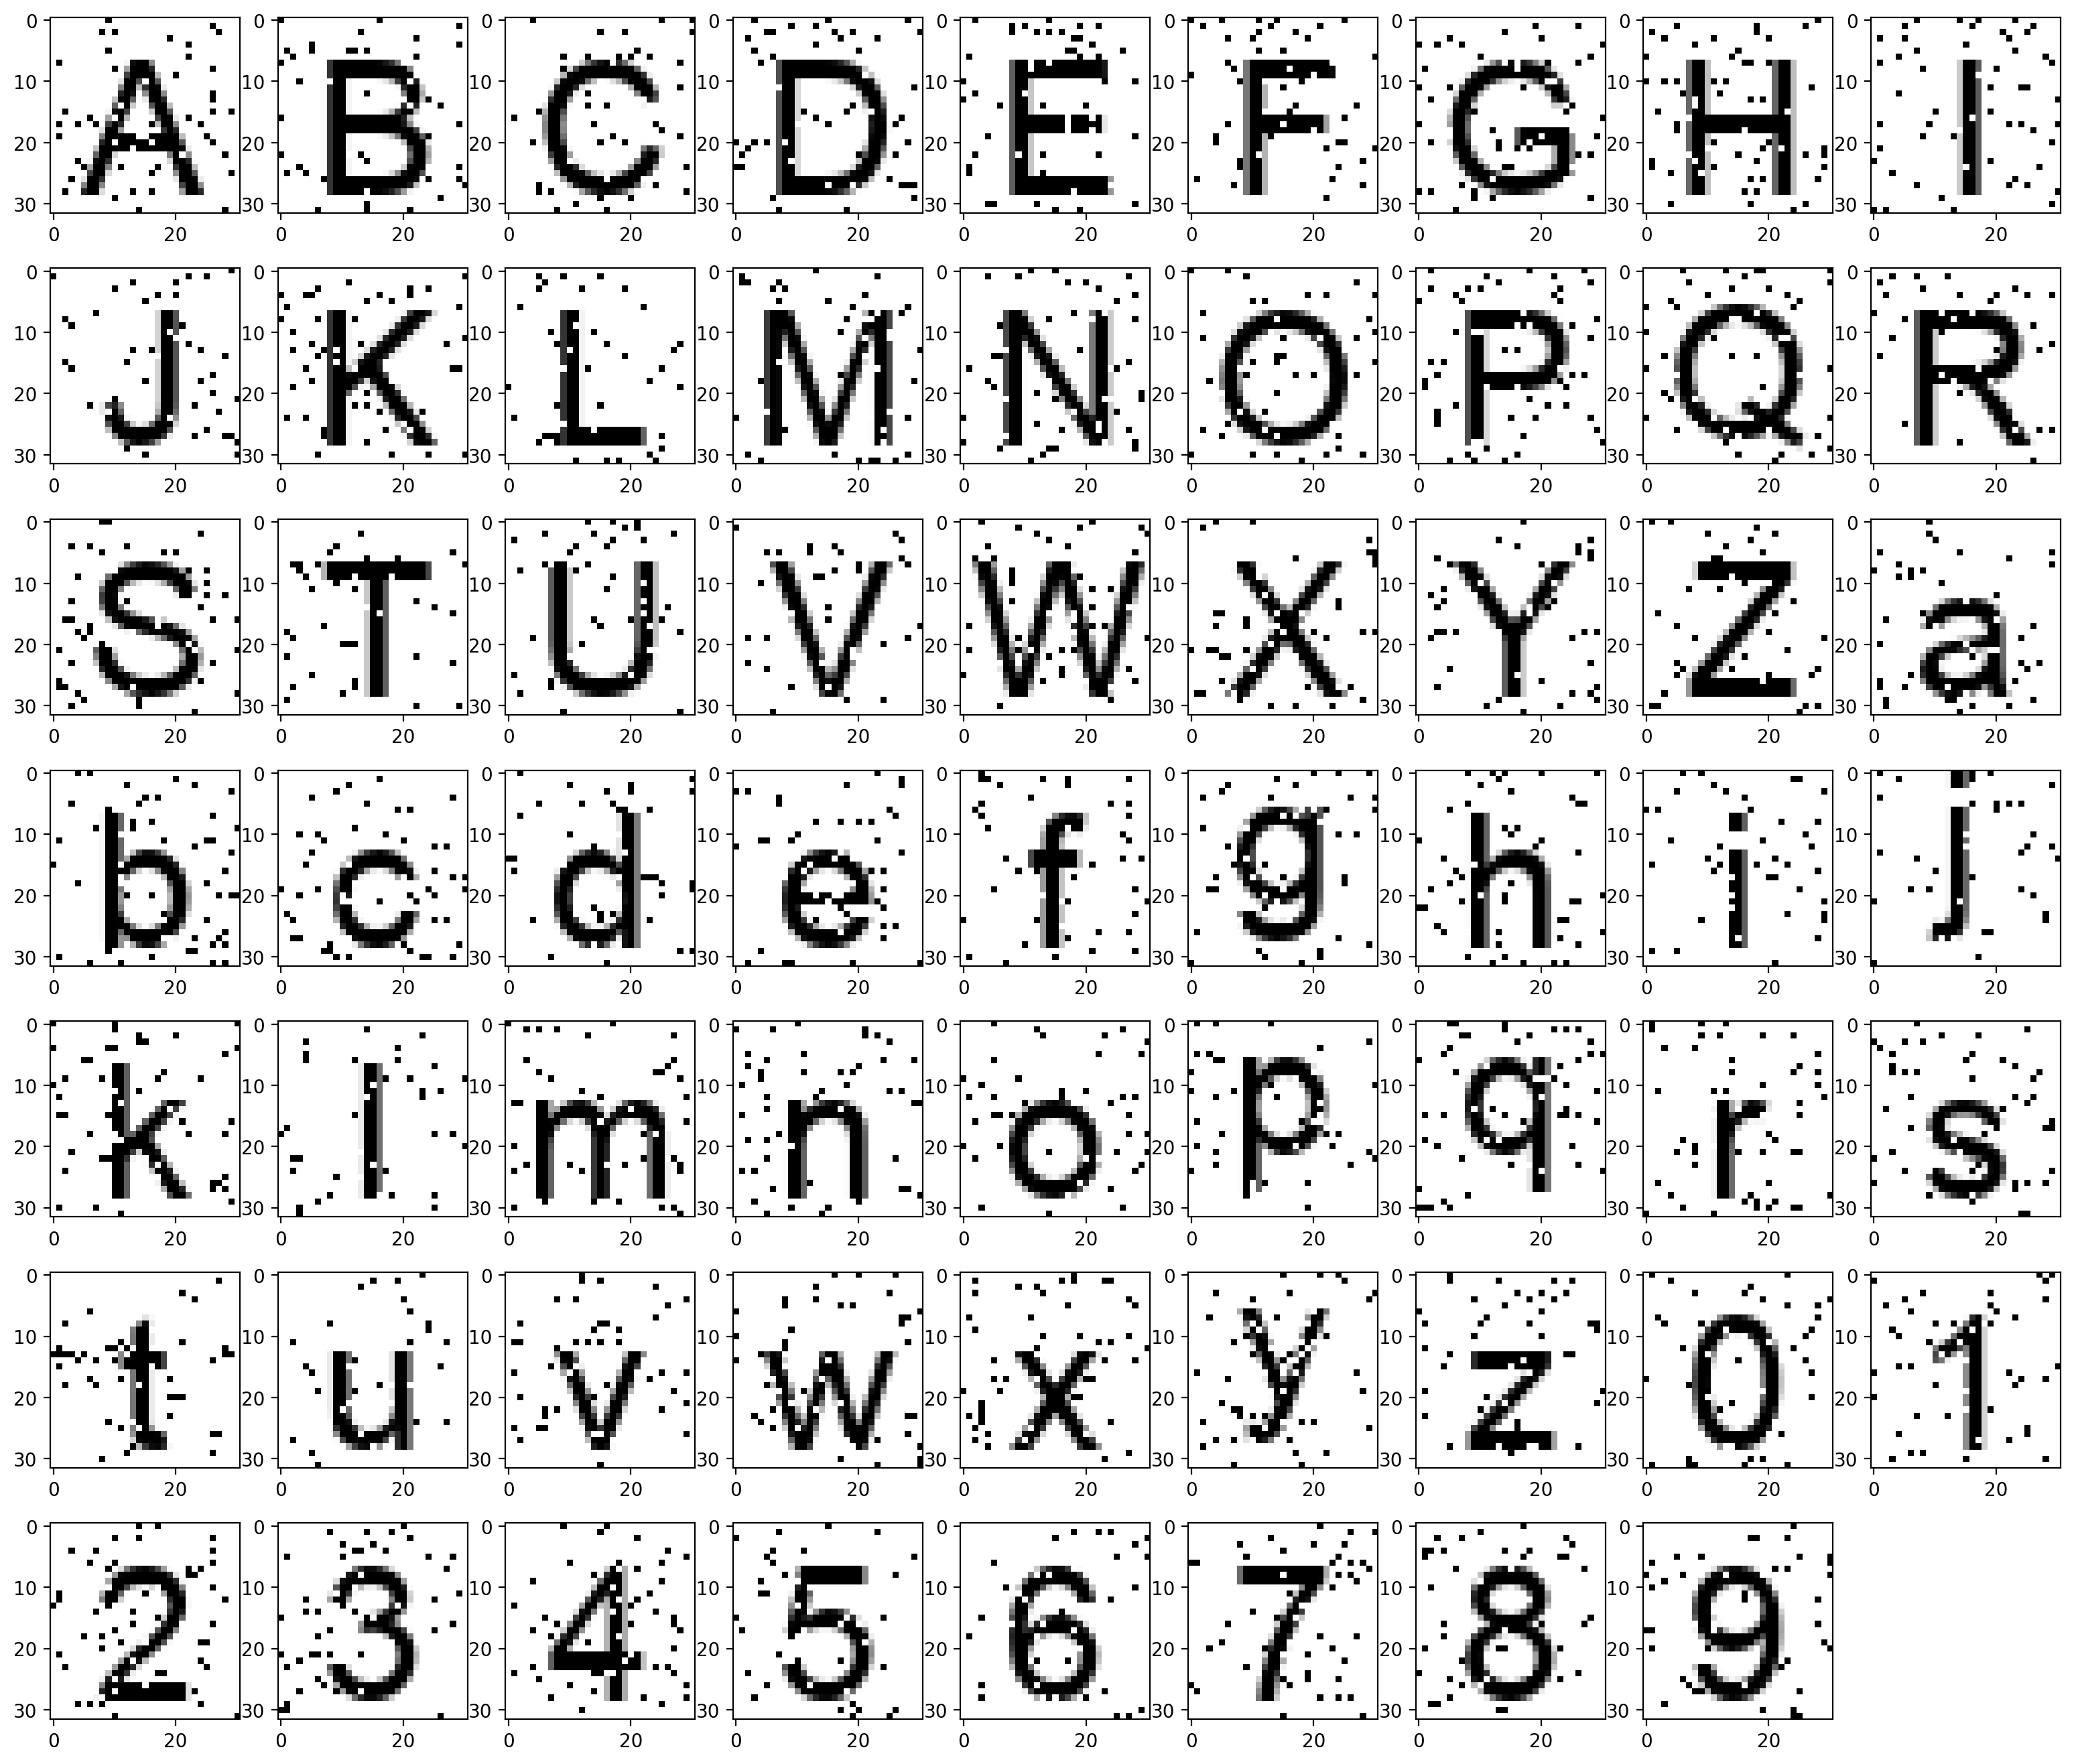
\includegraphics[width=\textwidth]{./images02/classification/groups.png}
\caption{One noisy image for each of the 62 classification groups.
\label{fig-classification-groups}}
\end{figure}

The association of images to groups was stored as sequences in SDM, as detailed by \citet{Kanerva1988} in Chapter 8. During the learning phase, the image bitstrings were stored pointing to their group's bitstrings, i.e., write(addr=bs\_image, datum=bs\_label). Thus, in order to classify an unknown image, we only had to read from its address and check which group has been found.

% TODO Add image showing the pointers.

During the learning phase, we have generated 100 noisy images for each character. The images had 5\% of noise, i.e., 5\% of their pixels have been randomly flipped. For example, see the generated images for letter A in Figure \ref{fig-classification-training-A}. Then, we have written the classification group bitstring into the bitstring associated to each noisy image, i.e., write(bs\_image, bs\_label). For a complete image training set, see Appendix XYZ.

\begin{figure}[!htb]
\centering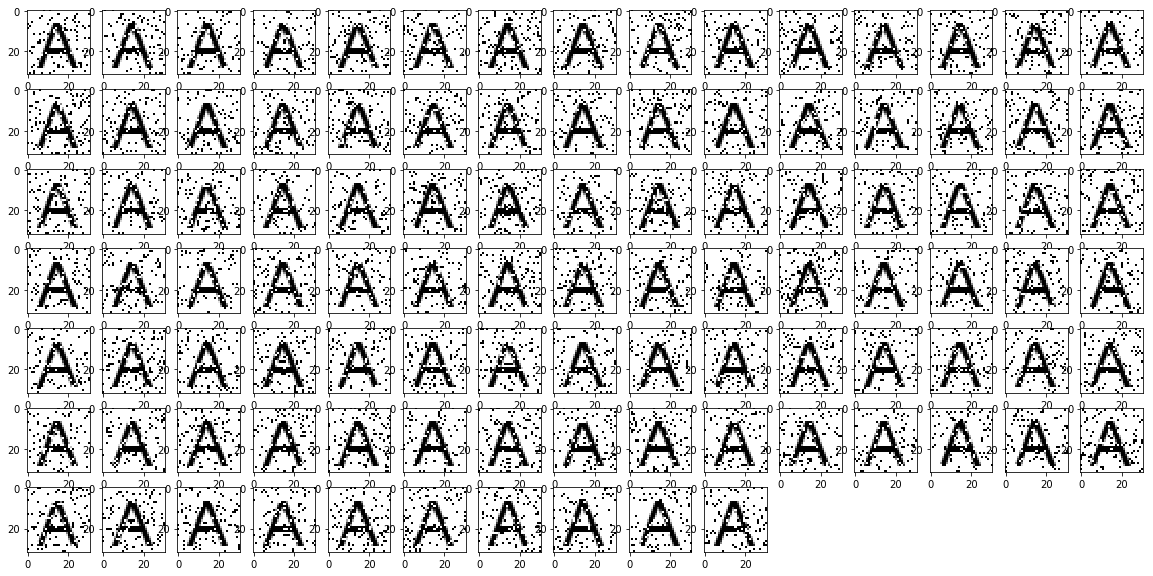
\includegraphics[width=\textwidth]{./images02/classification/trainingA.png}
\caption{100 noisy images generated to train label A.
\label{fig-classification-training-A}}
\end{figure}

Finally, we have assessed the performance of our classifier. We had done it in three different scenarios: high noise (20\%), low noise (5\%) and no noise. See Figures \ref{fig-classification-noise-high} and \ref{fig-classification-no-noise} for images with 20\% noise and no noise. The low noise scenario had the same noise as the training set. For each scenario, we had classified 620 unknown images with ten images per group.

\begin{figure}[!htb]
\centering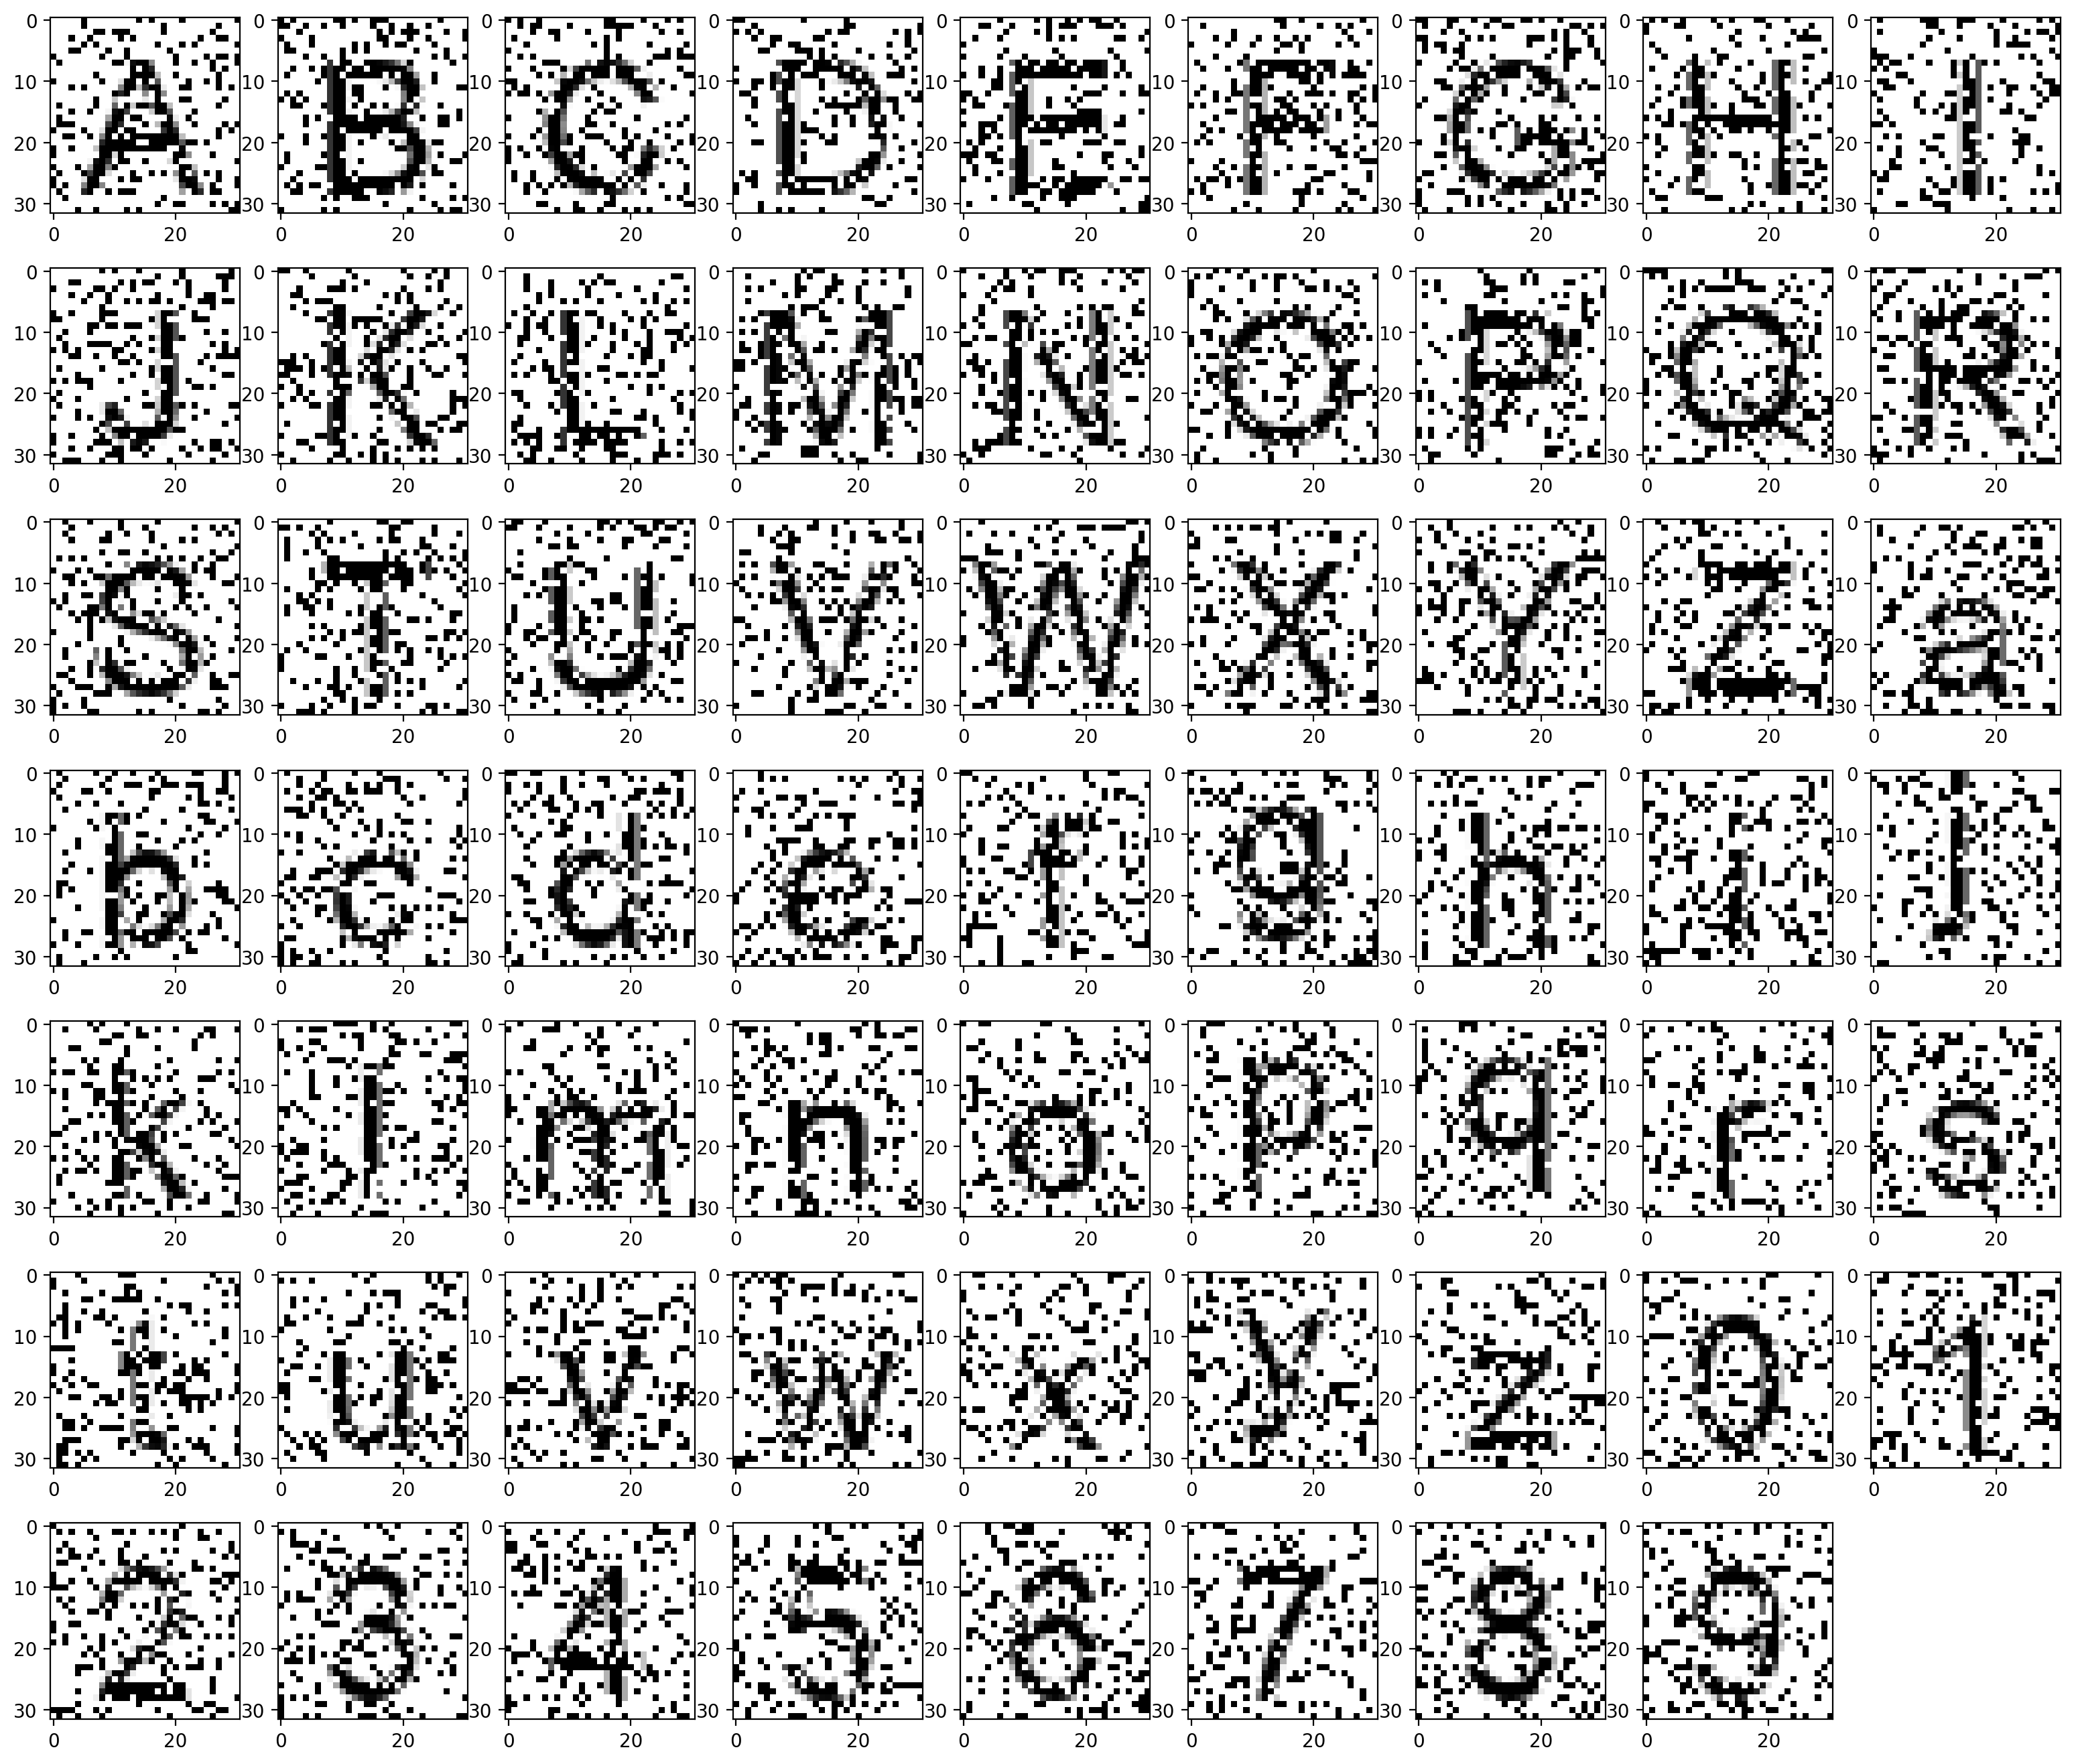
\includegraphics[width=0.75\textwidth]{./images02/classification/noise-high.png}
\caption{Images generated using a 20\% noise for the high noise scenario.
\label{fig-classification-noise-high}}
\end{figure}

\begin{figure}[!htb]
\centering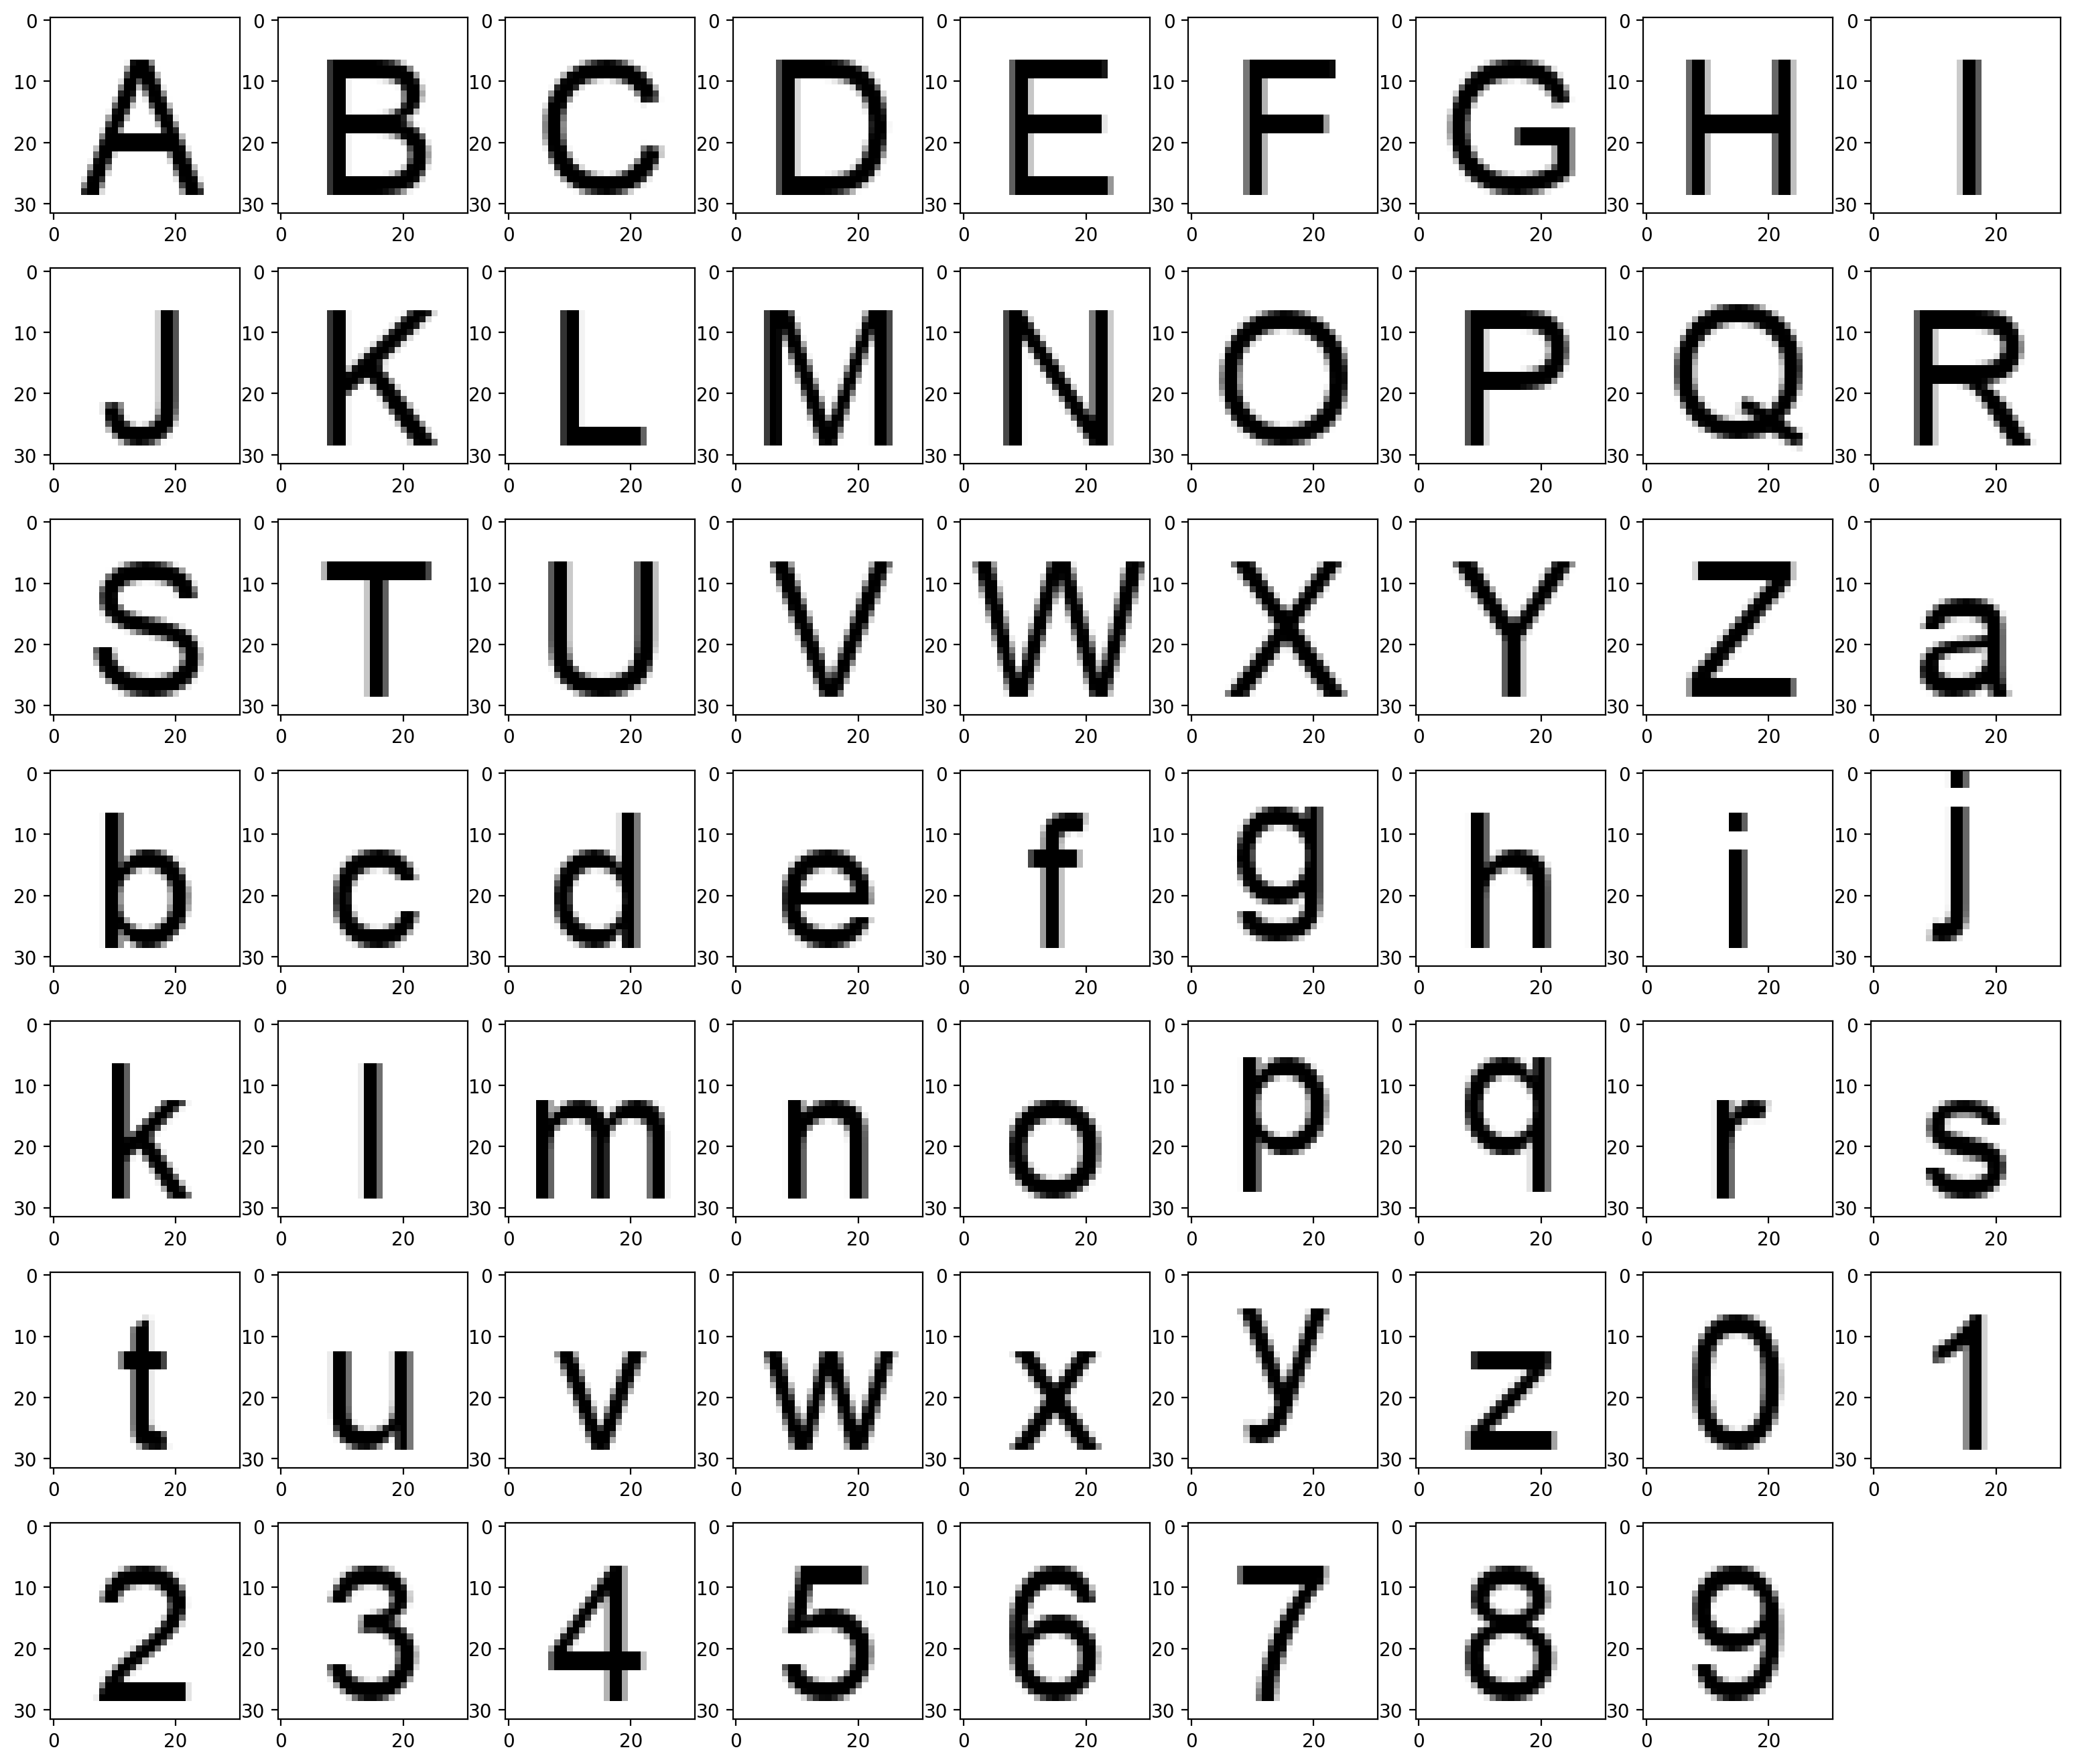
\includegraphics[width=0.75\textwidth]{./images02/classification/no-noise.png}
\caption{Images generated for the no noise scenario.
\label{fig-classification-no-noise}}
\end{figure}

The performance was calculated as the percentage of hits for each group. We did not expect the same performance for all groups because some groups become very similar to other depending on the noise level, and this similarity may even confuse a person (see Figure \ref{fig-classification-similarity}).

\begin{figure}[!htb]
  \centering
  \subfloat[``i'', ``l'', and ``r'' with 20\% noise.]{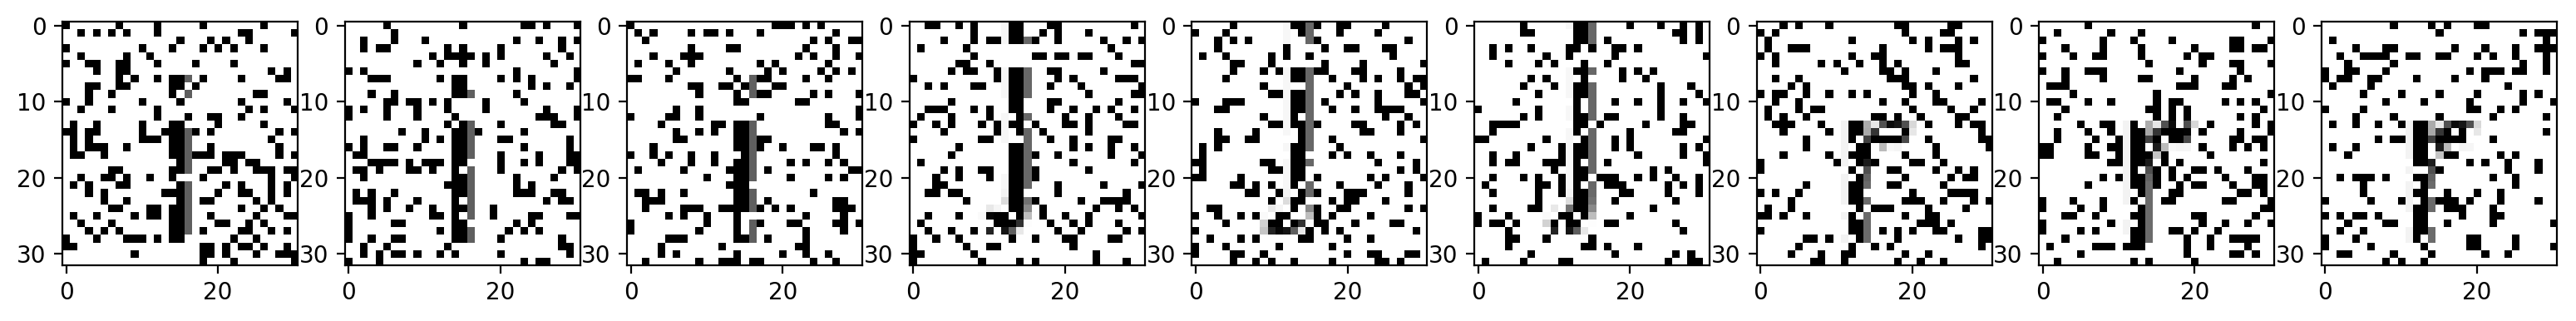
\includegraphics[width=\textwidth]{./images02/classification/ilr-high-noise.png}}

  \subfloat[``i'', ``l'', and ``r'' with 5\% noise.]{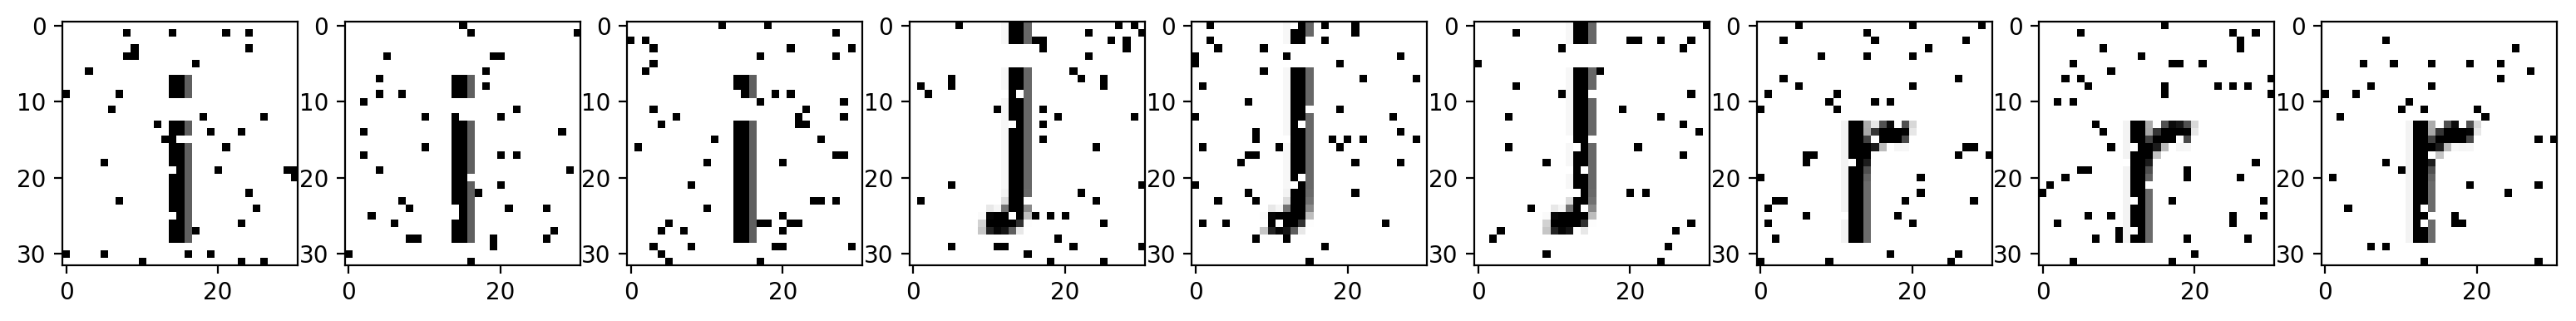
\includegraphics[width=\textwidth]{./images02/classification/ilr-low-noise.png}}

  \subfloat[``c'', ``d'', and ``o'' with 20\% noise.]{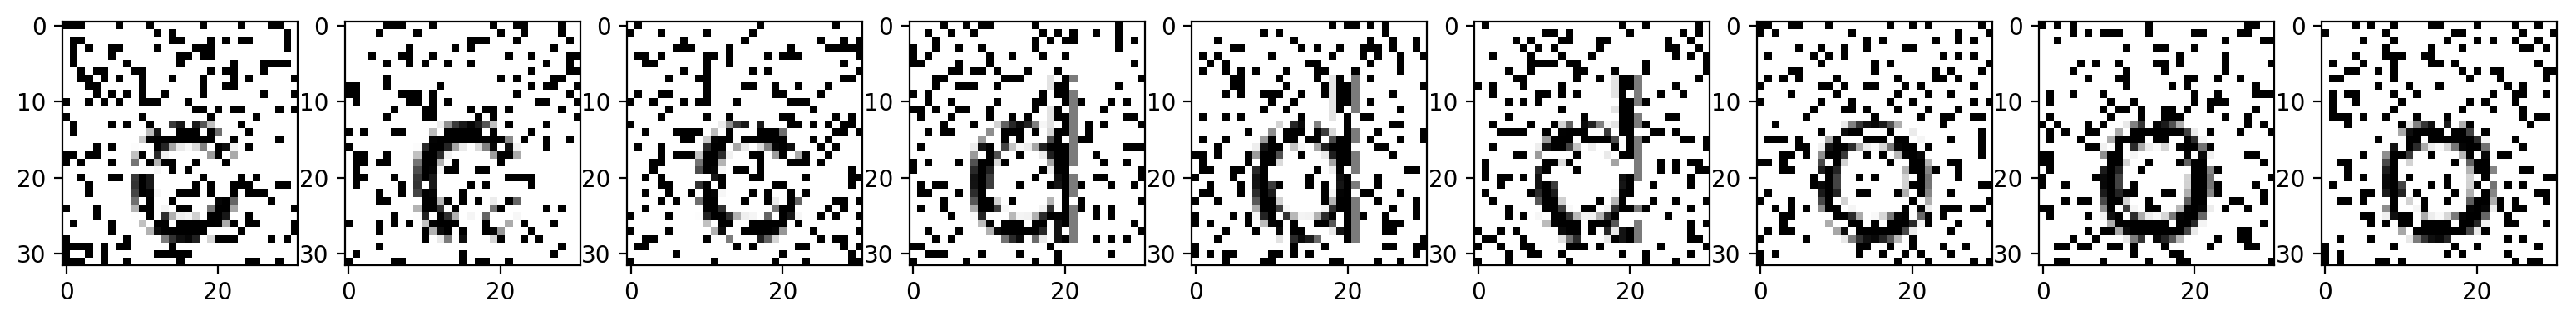
\includegraphics[width=\textwidth]{./images02/classification/cdo-high-noise.png}}

  \subfloat[``c'', ``d'', and ``o'' with 5\% noise.]{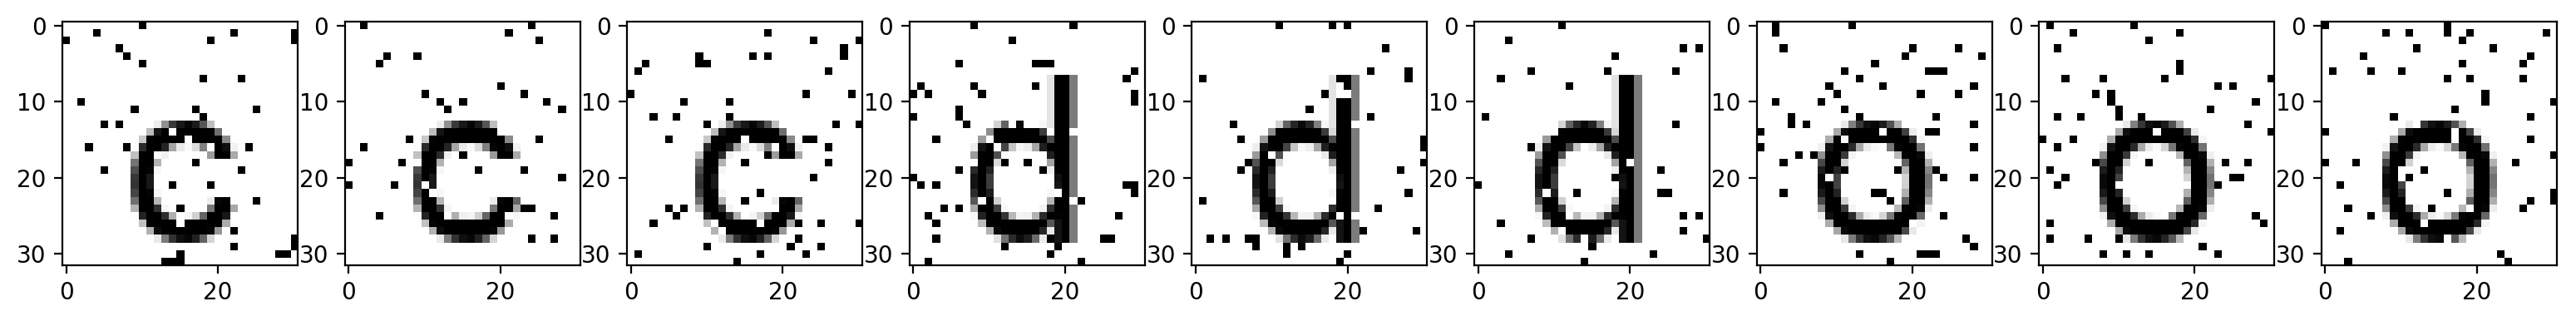
\includegraphics[width=\textwidth]{./images02/classification/cdo-low-noise.png}}

  \subfloat[``G'', ``O'', and ``Q'' with 20\% noise.]{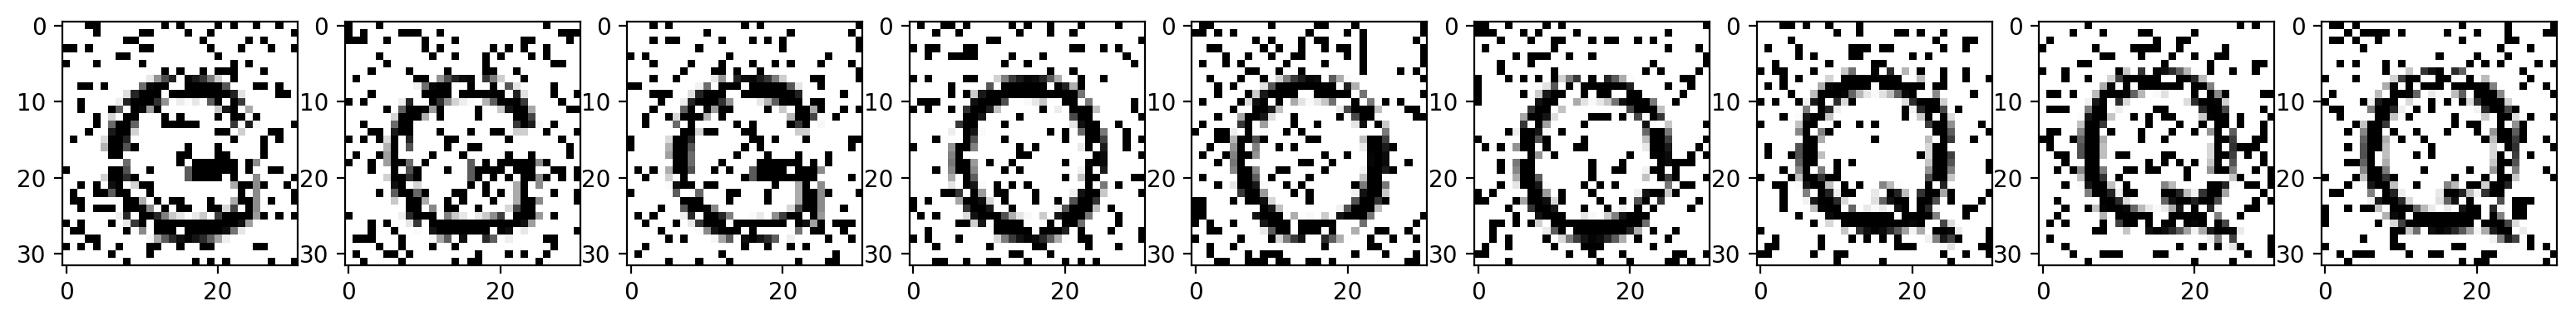
\includegraphics[width=\textwidth]{./images02/classification/GOQ-high-noise.png}}

  \subfloat[``G'', ``O'', and ``Q'' with 5\% noise.]{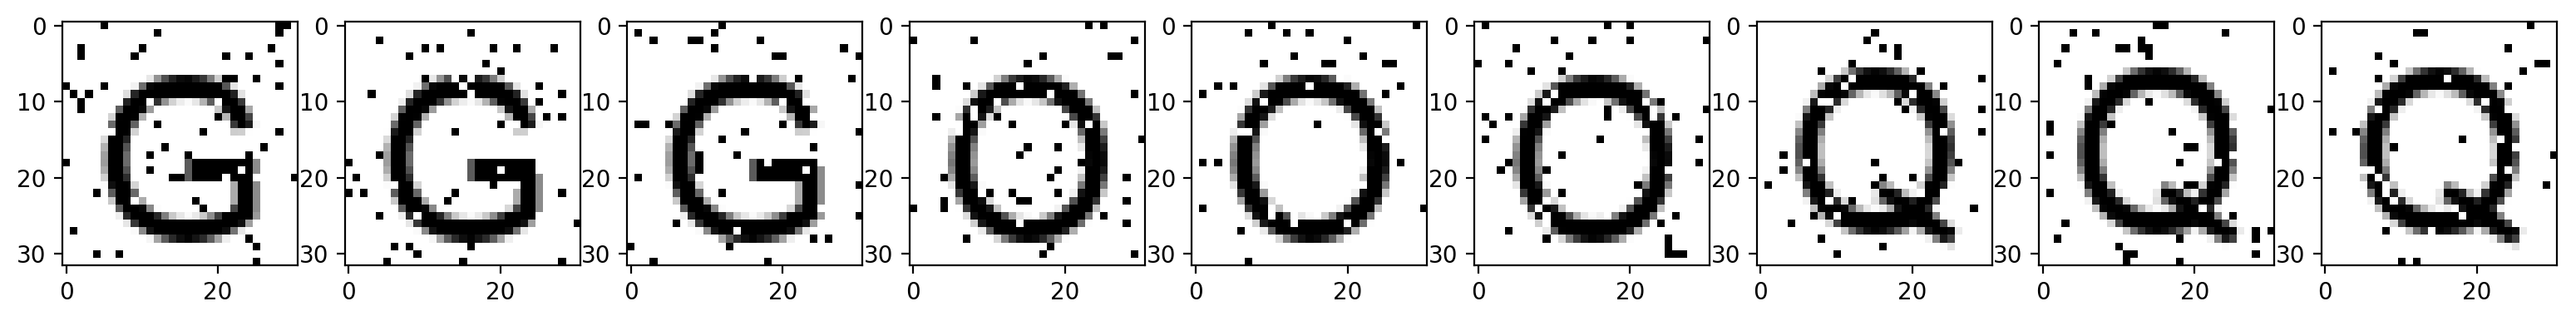
\includegraphics[width=\textwidth]{./images02/classification/GOQ-low-noise.png}}

  \caption{Images of different characters which may be confusing depending on the noise level.}
  \label{fig-classification-similarity}
\end{figure}

In the no noise scenario, the classifier has hit all characters, except letter ``l'' which was wrongly associated with the group of ``i''. We believe that it happened because the classifier had never seen an image with no noise and the difference between the images of ``l'' and ``i'' is smaller than the critical distance. So, both groups have been merged and it converged to only one of them. In our simulation, it happened to be the group of ``i''.

In the low noise scenario, it has made few mistakes. It correctly classified all images but some from characters ``b'', ``e'', ``f'', ``l'', ``t'', and ``9''. It completely classified ``l'' images to the ``i'' group. In the other cases, it made just a few mistakes. See Figure \ref{fig-classification-low-noise-results} to check the images and their classification.

\begin{figure}[!htb]
  \centering
  \subfloat[Images from character ``b which were classified as {[b, b, b, h, b, o, b, h, b, b]}, respectively. It has made 3 misses.]{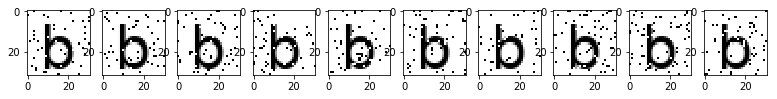
\includegraphics[width=\textwidth]{./images02/classification/low-noise-b.png}}

  \subfloat[Images from character ``e which were classified as {[e, e, e, e, e, e, e, e, o, e]}, respectively. It has made 1 miss. ]{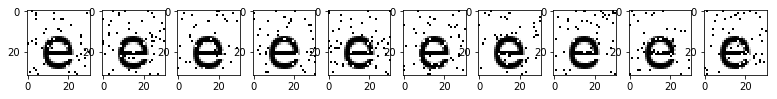
\includegraphics[width=\textwidth]{./images02/classification/low-noise-e.png}}

  \subfloat[Images from character ``f which were classified as {[i, f, f, I, I, I, f, f, f, f]}, respectively. It has made 4 misses. ]{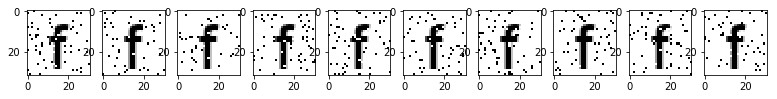
\includegraphics[width=\textwidth]{./images02/classification/low-noise-f.png}}

  \subfloat[Images from character ``l'' which were classified as {[i, i, i, i, i, i, i, i, i, i]}, respectively. It has missed them all as if both groups have been merged. ]{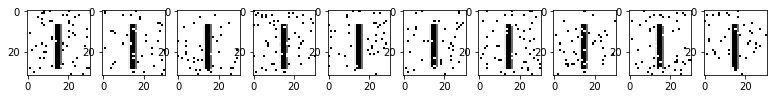
\includegraphics[width=\textwidth]{./images02/classification/low-noise-l.png}}

  \subfloat[Images from character ``t'' which were classified as {[t, t, t, t, t, t, t, i, t, t]}, respectively. It has made 1 miss. ]{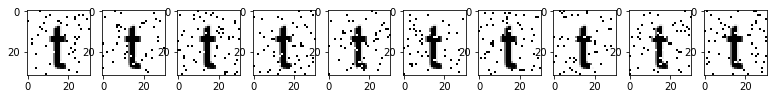
\includegraphics[width=\textwidth]{./images02/classification/low-noise-t.png}}

  \subfloat[Images from character ``9'' which were classified as {[9, 9, 0, 9, 9, 9, 0, 0, 9, 9]}, respectively. It has made 3 misses. ]{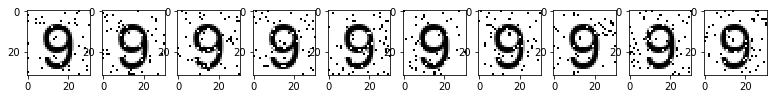
\includegraphics[width=\textwidth]{./images02/classification/low-noise-9.png}}

  \caption{Characters in the low noise scenario in which the classifier has made at least one mistake. In all the other cases, it correctly classified the images. We may notice that the groups of ``i'' and ``l'' have been completely merged by the classifier, because it cannot distinguish them, not even with no noise.}
  \label{fig-classification-low-noise-results}
\end{figure}

The high noise scenario is the most interesting, because, even in a high noise level, the classifier has hit most of the characters. It has hit all images for 44 out of 62 groups and made at least one miss for the other 18 groups. The misses may be seen in details in Figure \ref{fig-classificiation-high-noise-misses}.

\begin{figure}[!htb]
  \centering
  \subfloat[Images from character ``B'' which were classified as {[S, B, B, B, B, B, B, B, B, B]}. It has made 1 mistake. ]{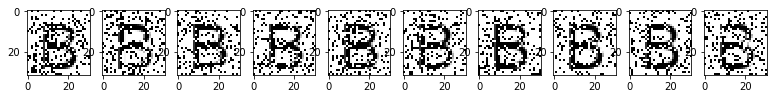
\includegraphics[width=\textwidth]{./images02/classification/high-noise-B.png}}

  \subfloat[Images from character ``O'' which were classified as {[G, G, O, O, O, O, O, O, O, O]}. It has made 2 mistakes. ]{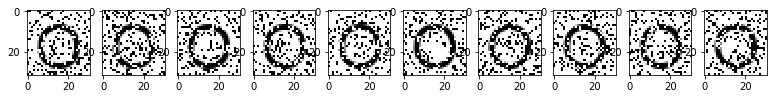
\includegraphics[width=\textwidth]{./images02/classification/high-noise-O.png}}

  \subfloat[Images from character ``T'' which were classified as {[T, T, T, T, T, I, T, T, T, T]}. It has made 1 mistake. ]{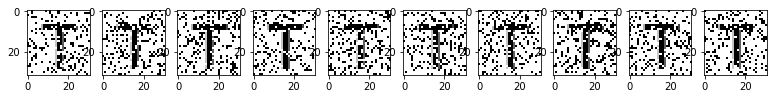
\includegraphics[width=\textwidth]{./images02/classification/high-noise-T.png}}

  \subfloat[Images from character ``Y'' which were classified as {[Y, I, Y, Y, Y, Y, Y, Y, Y, Y]}. It has made 1 mistake. ]{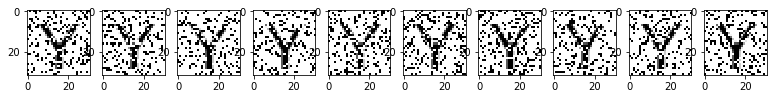
\includegraphics[width=\textwidth]{./images02/classification/high-noise-Y.png}}

  \subfloat[Images from character ``b'' which were classified as {[o, o, o, b, o, h, h, b, b, o]}. It has made 7 mistakes. ]{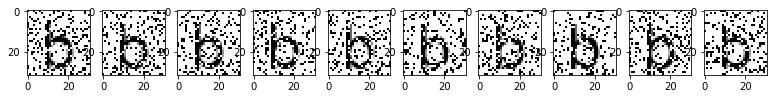
\includegraphics[width=\textwidth]{./images02/classification/high-noise-b2.png}}

  \subfloat[Images from character ``c'' which were classified as {[c, c, c, c, c, o, c, c, c, o]}. It has made 2 mistakes. ]{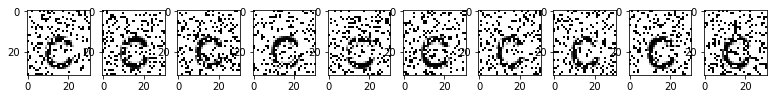
\includegraphics[width=\textwidth]{./images02/classification/high-noise-c.png}}

  \subfloat[Images from character ``e'' which were classified as {[e, o, e, o, o, o, e, o, o, e]}. It has made 6 mistakes. ]{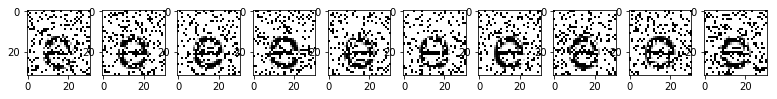
\includegraphics[width=\textwidth]{./images02/classification/high-noise-e.png}}

  \subfloat[Images from character ``f'' which were classified as {[I, I, I, I, i, I, I, I, I, I]}. It has missed them all. ]{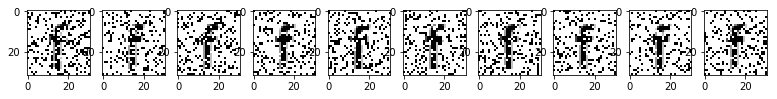
\includegraphics[width=\textwidth]{./images02/classification/high-noise-f.png}}

\end{figure}
\begin{figure}[!htb]\ContinuedFloat

  \subfloat[Images from character ``i'' which were classified as {[i, i, i, I, i, i, i, i, I, i]}. It has made 2 mistakes. ]{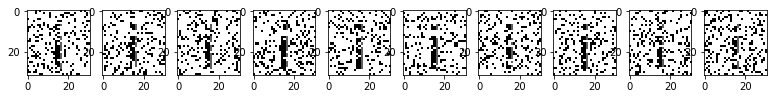
\includegraphics[width=\textwidth]{./images02/classification/high-noise-i.png}}

  \subfloat[Images from character ``j'' which were classified as {[j, j, j, I, I, j, j, j, j, I]}. It has made 3 mistakes. ]{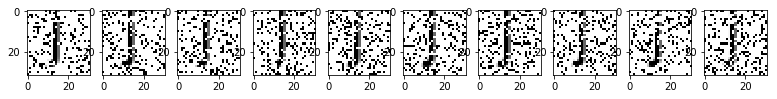
\includegraphics[width=\textwidth]{./images02/classification/high-noise-j.png}}

  \subfloat[Images from character ``l'' which were classified as {[I, i, I, I, I, I, i, I, I, i]}. It has missed them all. ]{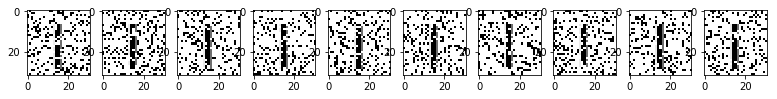
\includegraphics[width=\textwidth]{./images02/classification/high-noise-l.png}}

  \subfloat[Images from character ``n'' which were classified as {[u, n, n, n, n, n, u, u, u, h]}. It has made 5 mistakes. ]{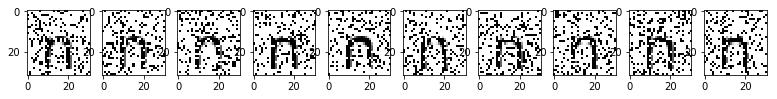
\includegraphics[width=\textwidth]{./images02/classification/high-noise-n.png}}

  \subfloat[Images from character ``q'' which were classified as {[q, q, q, q, q, q, q, q, q, g]}. It has made 1 mistake. ]{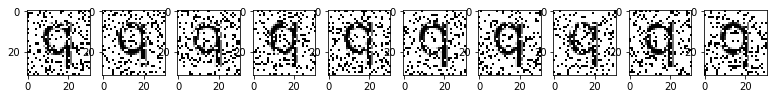
\includegraphics[width=\textwidth]{./images02/classification/high-noise-q.png}}

  \subfloat[Images from character ``t'' which were classified as {[I, r, I, i, I, i, i, i, I, i]}. It has missed them all. ]{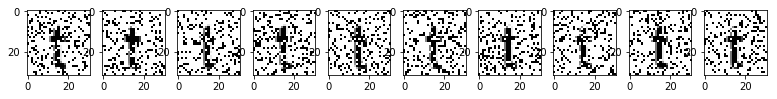
\includegraphics[width=\textwidth]{./images02/classification/high-noise-t2.png}}

  \subfloat[Images from character ``1'' which were classified as {[1, I, 1, I, 1, 1, I, I, 1, I]}. It has made 5 mistakes. ]{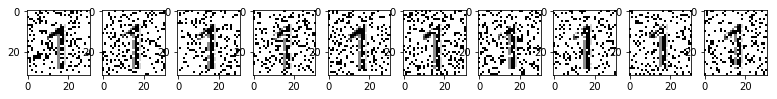
\includegraphics[width=\textwidth]{./images02/classification/high-noise-1.png}}

  \subfloat[Images from character ``7'' which were classified as {[7, 7, 7, I, 7, I, I, 7, 7, 7]}. It has made 3 mistakes. ]{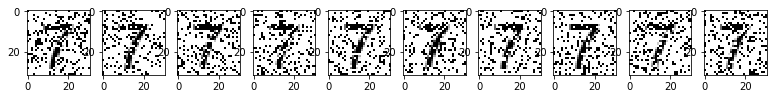
\includegraphics[width=\textwidth]{./images02/classification/high-noise-7.png}}

\end{figure}
\begin{figure}[!htb]\ContinuedFloat

  \subfloat[Images from character ``8'' which were classified as {[8, 6, 6, 6, 8, d, 8, 8, d, 6]}. It has made 6 mistakes. ]{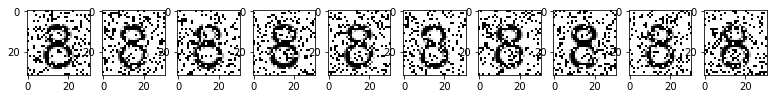
\includegraphics[width=\textwidth]{./images02/classification/high-noise-8.png}}

  \subfloat[Images from character ``9'' which were classified as {[9, 0, 6, 0, 9, 0, 0, 9, 0, 0]}. It has made 7 mistakes. ]{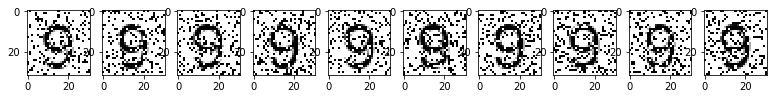
\includegraphics[width=\textwidth]{./images02/classification/high-noise-9.png}}

  \caption{Characters in the high noise scenario in which the classifier has made at least one mistake. In all the other cases, it correctly classified the images.}
  \label{fig-classification-high-noise-misses}
\end{figure}

The critical distance plays an important role in the classification error. As we have 62 groups and each has been trained with 100 images, there were 6,200 writes to the memory. When an image is being classified, it will have to converge to a group, and the convergence depends on the distance between this image and the images from the training set, i.e., in the noise level.

In our simplified scenario, there is neither translation nor rotation. Future work may explore how sensible this classification algorithm is to these operations. We expect that, with proper training, the algorithm will remain classifying the images with a good hit rate.

These results show that the SDM may be used as a supervised classification algorithm. Although we do not believe that the mapping between images and bitstrings are even close to the way human cognition deals with images, we believe the results are exciting and useful to many possible real-world problems.













\chapter{Results (vii): Image noise filtering application}

\lstset{
    language=Python,
    basicstyle=\small\ttfamily,
}

Image noise filtering consists in removing the noise from an input, in our case an image. Our images are black \& white images, and the noise is generated randomly flipping some of their pixels from black to while and vice versa. In Figure \ref{fig-filter-progressive-noise}, we may see an image with different levels of noise, from 0\% to 45\% in steps of 5\%. It makes no sense to apply 50\% of noise because it would absolutely randomize the image.

\begin{figure}[!htb]
\centering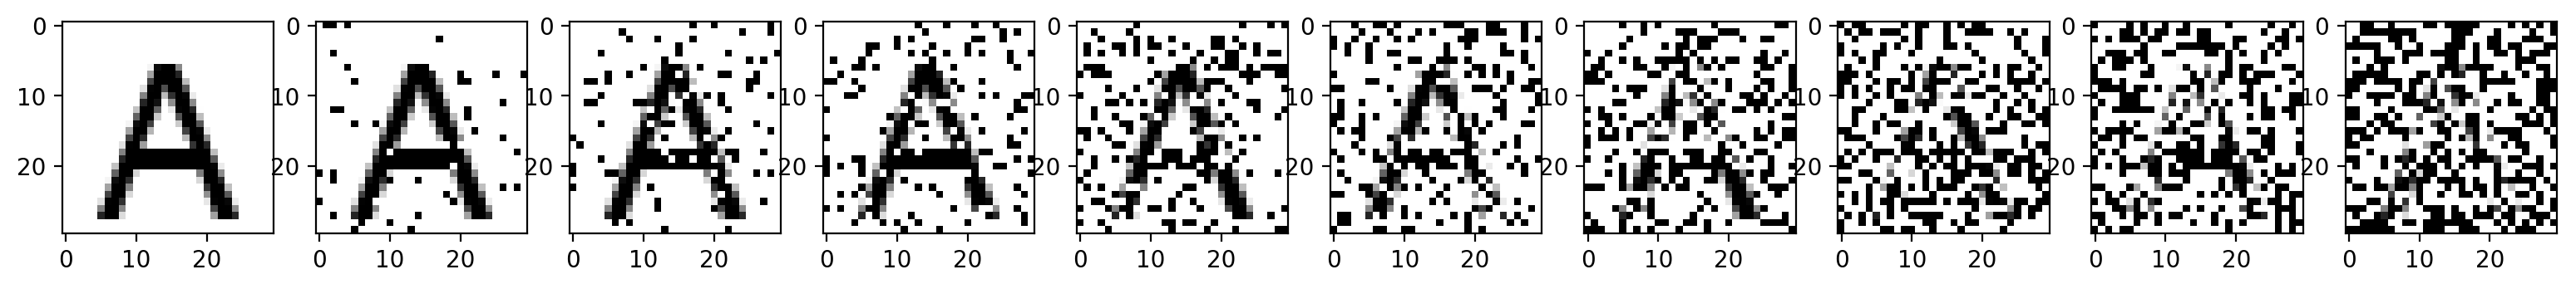
\includegraphics[width=\textwidth]{./images02/filter/progressive-noise.png}
\caption{Progressive noise into letter ``A'', from 0\% to 45\% in steps of 5\%.
\label{fig-filter-progressive-noise}}
\end{figure}

The images have 30 x 30 pixels, totaling 900 pixels per image. Each image is mapped into a bitstring of 1,000 bit in which the bits are set according to the color of each pixel of the image. White pixels are assigned to bit 0, and black pixels to bit 1. The 100 remaining bits are all set to zero. This is a bijective mapping (or one-to-one) from images and bitstrings, i.e., there is one, and only one, bitstring for each image, and vice versa.

In the learning phase, 200 noisy images were generated and written into SDM. Half of the letter ``I'' and half of the letter ``T'' (see Figure \ref{fig:filter-training}). They were written into their own addresses, i.e., \lstinline{write(address=bs_image, datum=bs_image)}.

\begin{figure}[!htb]
  \subfloat[Letter ``I'' with 15\% of noise. ]{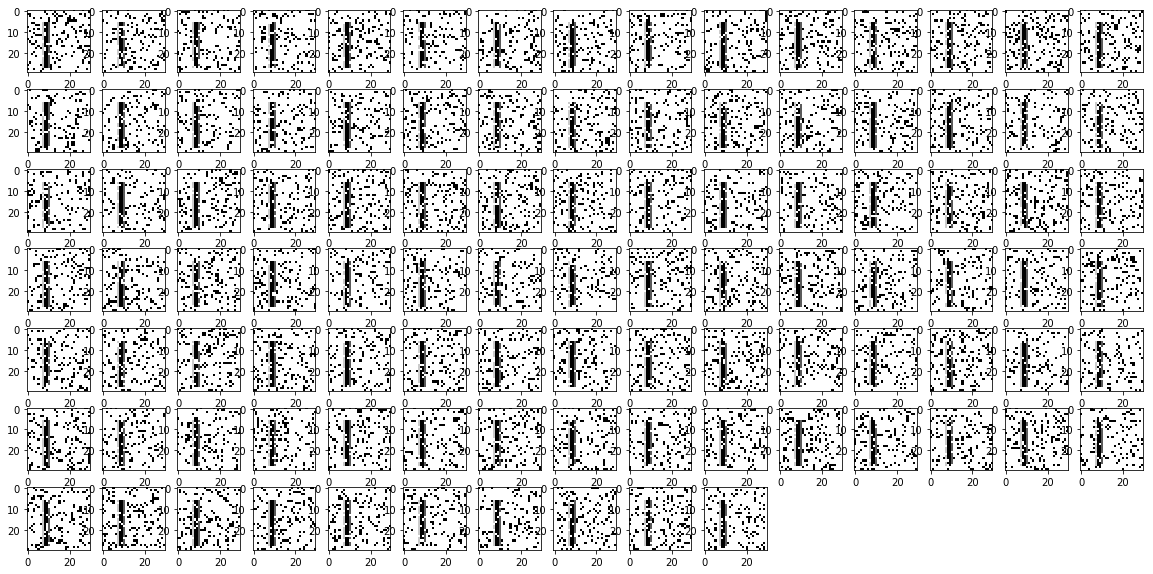
\includegraphics[width=\textwidth]{./images02/filter/training-i.png}}

  \subfloat[Letter ``T'' with 15\% of noise. ]{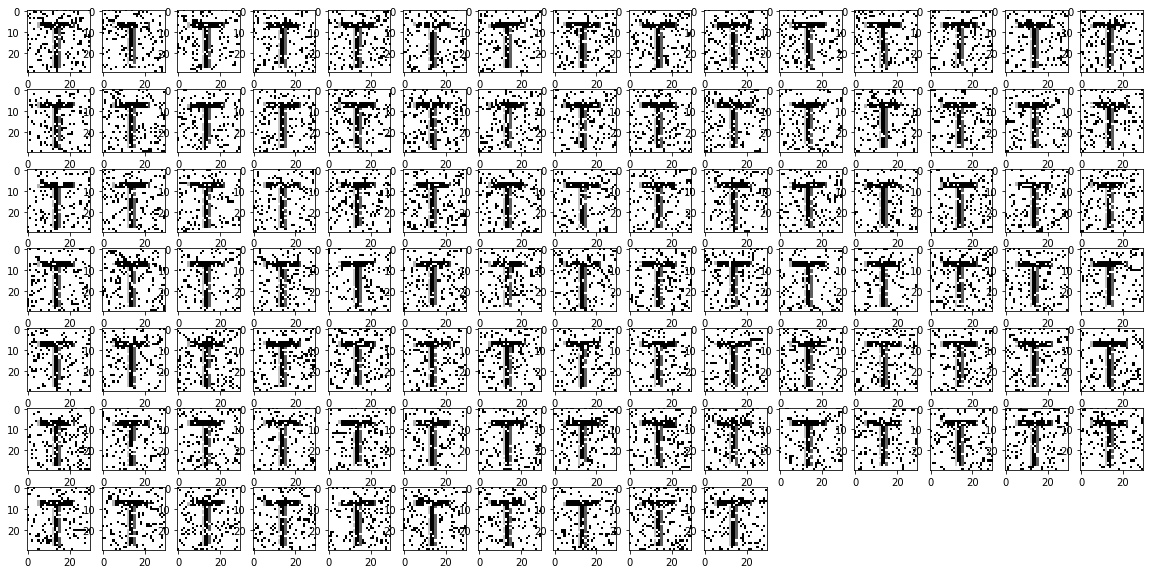
\includegraphics[width=\textwidth]{./images02/filter/training-t.png}}

  \caption{Training images written into the SDM. They were written in their own addresses --- write(address=bs\_image, datum=bs\_image).}
  \label{fig:filter-training}
\end{figure}

Then, in order to test the filtering, we just have read from noisy images, and the results were remarkable. We were able to clean images up to 42\% of noise (see Figure \ref{fig:filter-testing}). While SDM has never seen a clean version of the letters, it just learned from the learning phase which pixels have appeared more frequently and choose them.

\begin{figure}[!htb]
  \subfloat[Steps of reading from letter ``T'' with 42\% of noise]{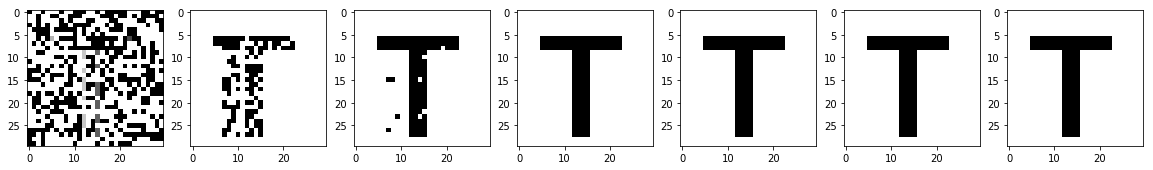
\includegraphics[width=\textwidth]{./images02/filter/T-42noise.png}}

  \subfloat[Steps of reading from letter ``I'' with 42\% of noise]{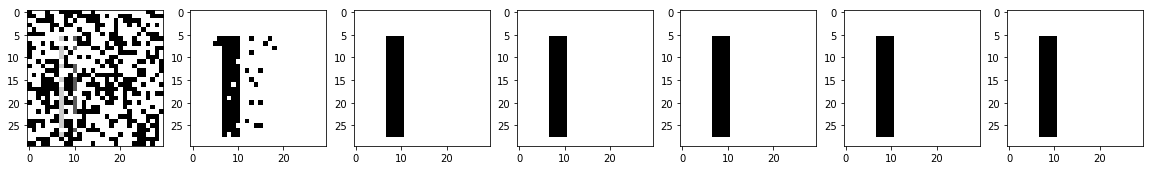
\includegraphics[width=\textwidth]{./images02/filter/I-42noise.png}}

  \caption{In order to test the SDM as a noise filter, we read from noisy images expecting to get a clean image. It is interesting to highlight that SDM has never seen a clean version letters ``T'' and ``I''.
  \label{fig:filter-testing}
  }
\end{figure}

A simplified mathematical analysis would be: During the learning phase, $200$ images with 15\% of noise were written to SDM, so, the average distance between them and the clean image was 150 bits. Thus they shared, on average, 175 hard locations with the clean image. In these 175 hard locations, the counter's value for a black pixel mapped to bit 1 was $(1-0.15) \cdot 200 - 0.15 \cdot 200 = 140$. Finally, let's analyze the reading. When reading from a noisy image with 42\% of noise, the average distance between the noisy image and its clean image is 420, which means they share, on average, 6 hard locations. As the average number of activated hard locations is 1,072, the sum of their counters will be, on average, $Y = 6 \cdot 140 - \sum_{i=1}^{1072-6} X_i$, where $X_i$ is a Bernoulli trial with probability 0.5. Hence, $P(\text{black pixel}) = P(Y > 0) = P(6 \cdot 140 - \sum_{i=1}^{1072-6} X_i > 0) = P(\sum_{i=1}^{1066} X_i < 840) = 99.99\%$. But, when reading from a noisy image with 45\% of noise, the average number of hard locations shared with the clean image is only 3. Thus the sum of the activated hard locations' counters will be, on average, $3 \cdot 140 - \sum_{i=1}^{1072-3} X_i$, and $P(\text{black pixel}) = P(\sum_{i=1}^{1069} X_i < 420) = 1.28 \cdot 10^{-12}$. The probability abruptly drops from 100\% to 0\% when the noise goes from 42\% to 45\% (see Figure \ref{fig:filter-prob-right-pixel}). The analysis for while pixels is exactly the same, but with opposite signs. The code to calculate this probability is available in ``Noise filter - Math analysis'' notebook \citep{sdmframework}.

This is a simplified analysis because it does not take into consideration the hard locations shared by the different letters. It works fine for our example because letters ``I'' and ``T'' are almost orthogonal and share, on average, only one hard location.

\begin{figure}[!htb]
\centering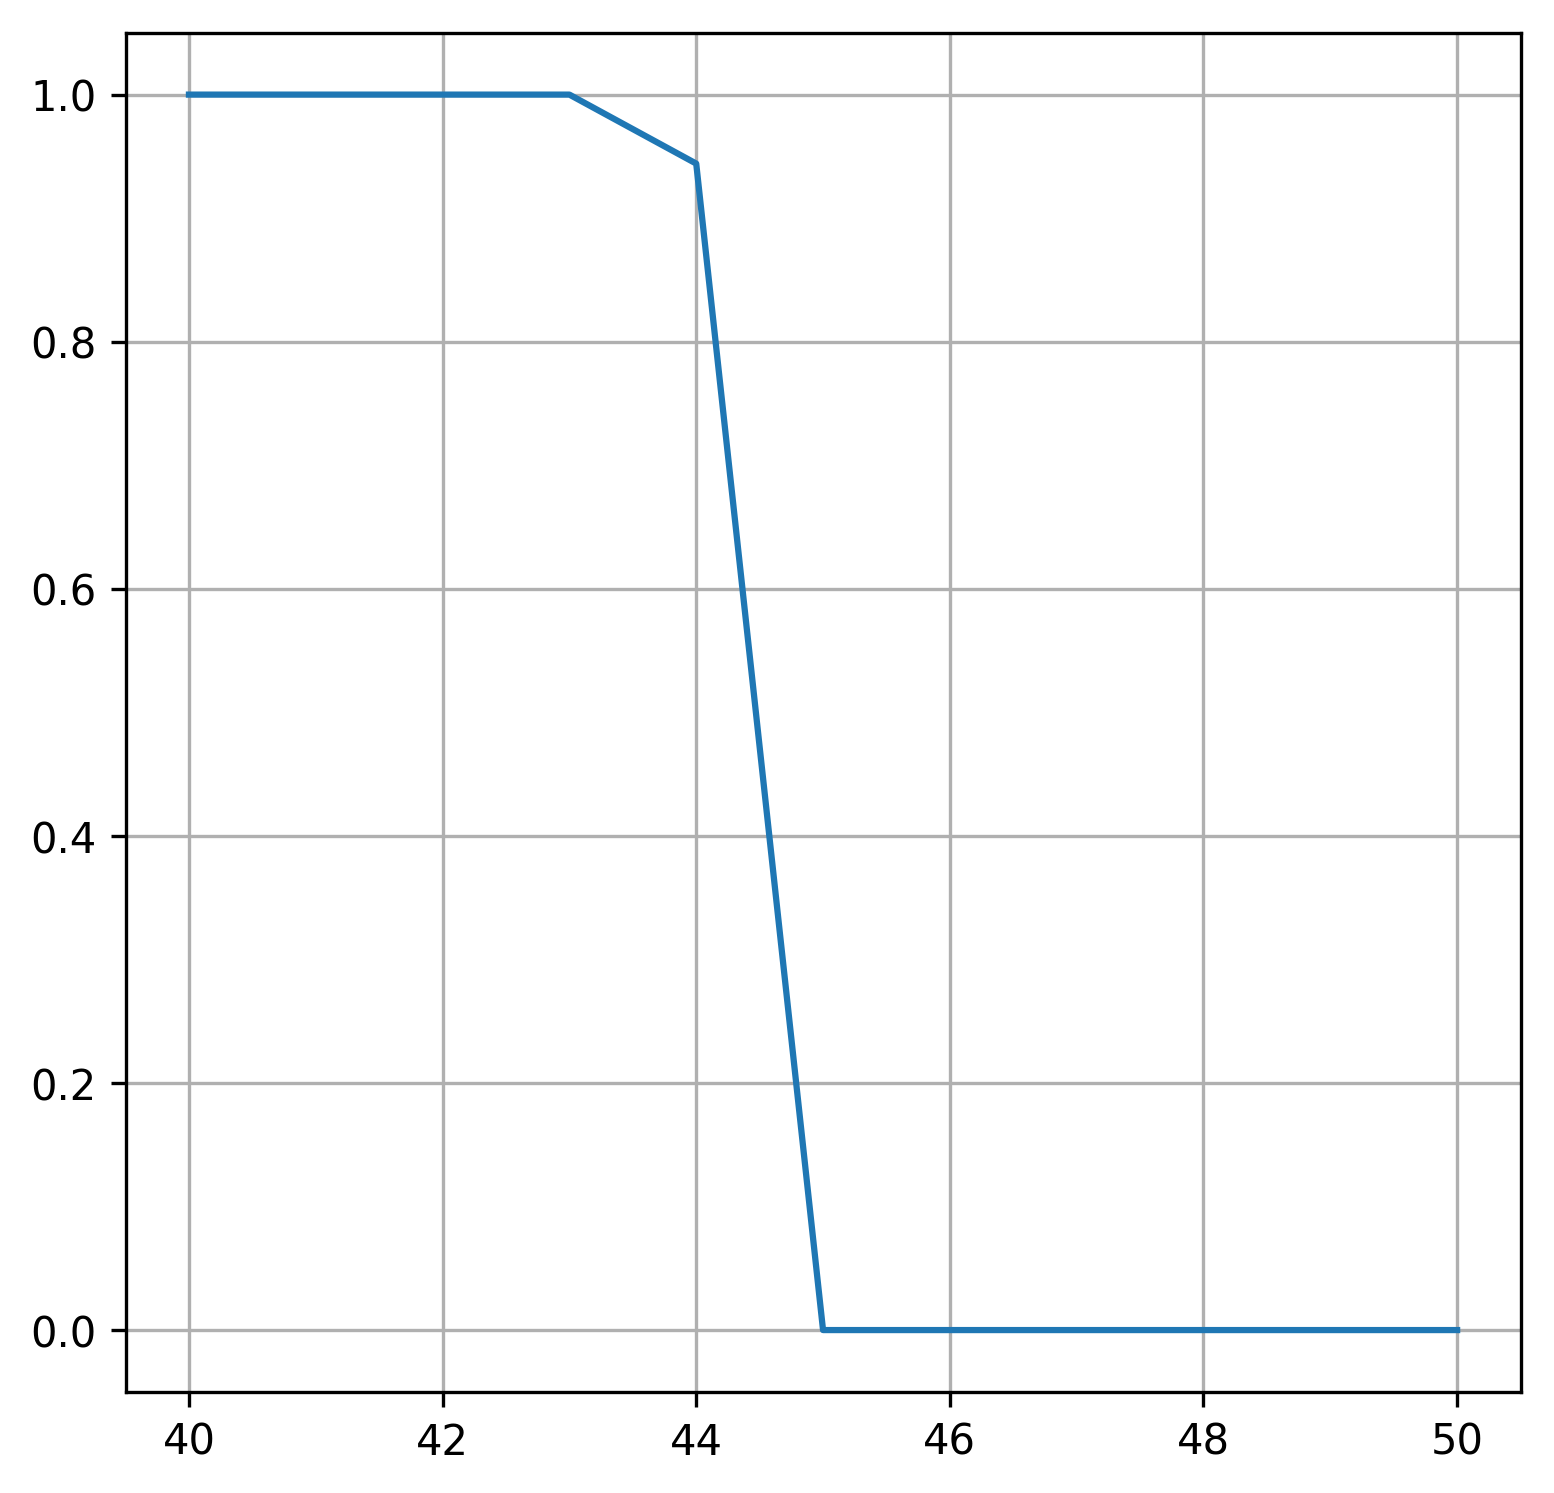
\includegraphics[width=0.7\textwidth]{./images02/filter/prob-right-pixel.png}
\caption{Probability of getting the right pixel when reading from an image with noise $p$. It assumes that SDM was trained with 200 images with 15\% noise.
\label{fig:filter-prob-right-pixel}
}
\end{figure}

If the intersection between images becomes too high, the noise filter stops working properly. We have confirmed it writing the letters ``B'', ``C'', ``D'' and the numeral ``8''. They share a high number of hard locations, and our noise filter could not filter their noise correctly. The training sets can be seen in Figure \ref{fig:filter-training2} and the results in Figure \ref{fig:filter-results2}.

\begin{figure}[!htb]
  \subfloat[Letter ``B'' with 15\% of noise. ]{\includegraphics[width=0.5\textwidth]{./images02/filter/training2-b.png}}
  \subfloat[Letter ``C'' with 15\% of noise. ]{\includegraphics[width=0.5\textwidth]{./images02/filter/training2-c.png}}

  \subfloat[Letter ``D'' with 15\% of noise. ]{\includegraphics[width=0.5\textwidth]{./images02/filter/training2-d.png}}
  \subfloat[Letter ``8'' with 15\% of noise. ]{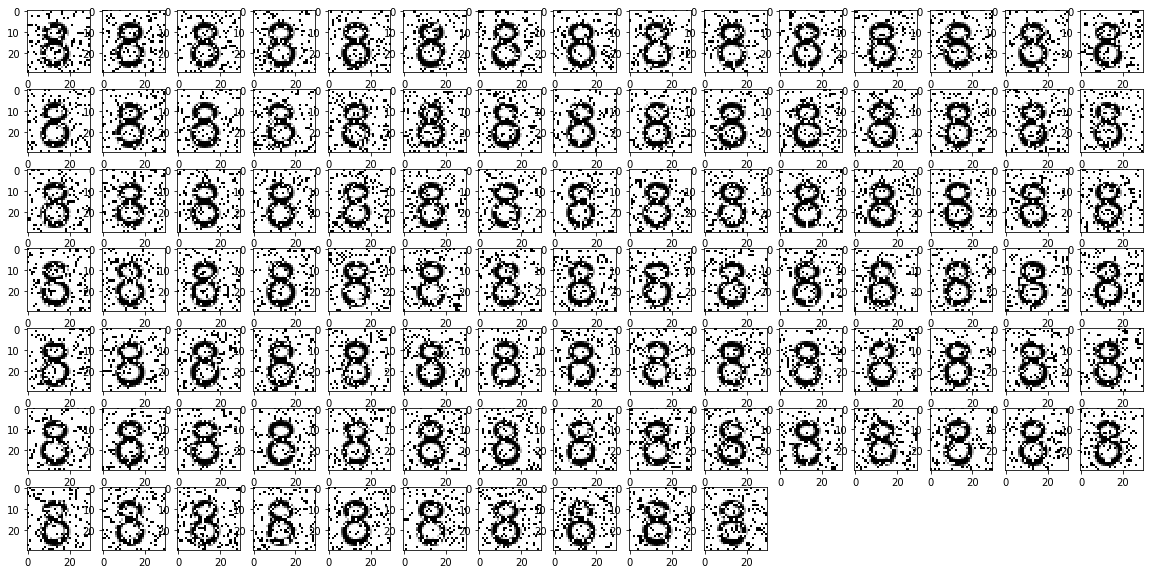
\includegraphics[width=0.5\textwidth]{./images02/filter/training2-8.png}}

  \caption{Training images in which the intersection between images is too high. They were written in their own addresses --- write(address=bs\_image, datum=bs\_image).}
  \label{fig:filter-training2}
\end{figure}

\begin{figure}[!htb]
  \captionsetup[subfigure]{labelformat=empty}
  \subfloat[]{\includegraphics[width=0.285\textwidth]{./images02/filter/case2-b-10noise.png}}

  \subfloat[]{\includegraphics[width=0.57\textwidth]{./images02/filter/case2-c-10noise.png}}

  \subfloat[]{\includegraphics[width=0.285\textwidth]{./images02/filter/case2-d-10noise.png}}

  \subfloat[]{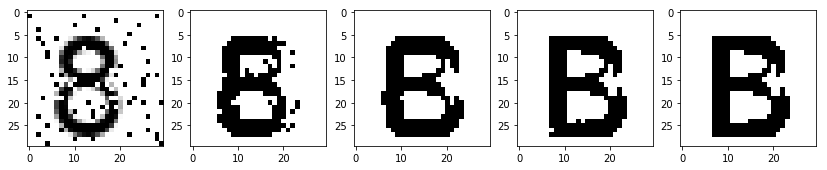
\includegraphics[width=0.57\textwidth]{./images02/filter/case2-8-10noise.png}}

  \caption{When the intersection between images becomes too high, there appears some interference in the resulting image. All cases have 10\% noise. We can notice that the empty space on the right side of the ``C'' letter generates some white pixels on the right side of both ``B'' and ``D'' letters.
  \label{fig:filter-results2}
  }
\end{figure}

A possible solution to this interference problem is to use labels. Each label has a random bitstring, which will be chunked with the images before writing into SDM. Hence, before reading, we also have to chunk the image with the label --- which means we need to know the label of each image. The chunk was done using the exclusive OR (XOR) operator, i.e., $bs\_chunck = bs\_image \oplus bs\_label$. In other words, we run \lstinline{write(address=bs_chunk, datum=bs_label)} during the training, and \lstinline{read(address=bs_chunk)} during the testing. We used the same training set as before, and the results can be seen in Figure \ref{fig:filter-results2-chunk}.

\begin{figure}[!tb]
  \captionsetup[subfigure]{labelformat=empty}
  \subfloat[]{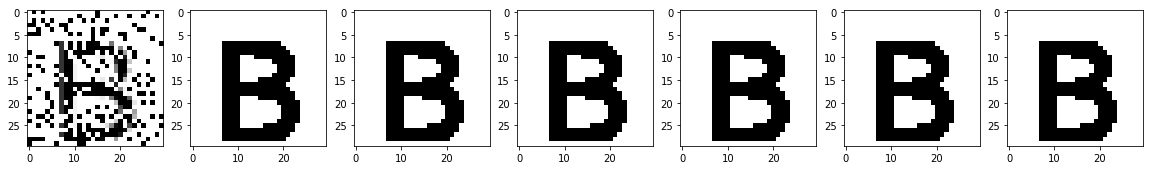
\includegraphics[width=\textwidth]{./images02/filter/labelB-20noise.png}}

  \subfloat[]{\includegraphics[width=\textwidth]{./images02/filter/labelC-20noise.png}}

  \subfloat[]{\includegraphics[width=\textwidth]{./images02/filter/labelD-20noise.png}}

  \subfloat[]{\includegraphics[width=\textwidth]{./images02/filter/label8-20noise.png}}

  \caption{Using labels solves the interference problem when the intersection between images becomes too high. All cases have 20\% noise.
  \label{fig:filter-results2-chunk}
  }
\end{figure}

The chunk through exclusive OR (XOR) works because of Theorem \ref{thm:xor-chuncks}, which says that chunking the images with labels will generate, on average, orthogonal bitstrings. Thus, these orthogonal bitstrings will not interfere with each other because they share, on average, only one hard location.

The disadvantage of using labels is that it requires classification of the images. In our example, we just used the correct label with each image, but we could have used our classification algorithm as a pre-processing step, and only then run the noise filter.

\begin{theorem}
If $v_1$ and $v_2$ are random bitstrings, then $\forall a, b, \mathbf{E} \left[ d(a \oplus v_1, b \oplus v_2) \right] = n/2$.
\label{thm:xor-chuncks}
\end{theorem}
\begin{proof}
Let $\mathbb{A} = \{ i | a^i = b^i \}$ be the indexes in which the bits of $a$ are equal to the bits of $b$, and $\mathbb{B} = \{ i | a^i \ne b^i \}$ be indexes in which the bits of $a$ are different from the bits of $b$. Thus,

\begin{align*}
d(a \oplus v_1, b \oplus v_2) &= \sum_{i=1}^n d(a^i \oplus v_1^i, b^i \oplus v_2^i) \\
    &= \sum_{i=1}^n (a^i \oplus v_1^i) \oplus (b^i \oplus v_2^i) \\
    &= \sum_{i=1}^n (a^i \oplus b^i) \oplus (v_1^i \oplus v_2^i) \\
    &= \sum_{i \in \mathbb{A}} (a^i \oplus b^i) \oplus (v_1^i \oplus v_2^i) +
       \sum_{i \in \mathbb{B}} (a^i \oplus b^i) \oplus (v_1^i \oplus v_2^i)
\end{align*}

For $i \in \mathbb{A}$, $a^i \oplus b^i = 0$, and follows:

\begin{align*}
(a^i \oplus b^i) \oplus (v_1^i \oplus v_2^i) &= 0 \oplus (v_1^i \oplus v_2^i) \\
    &= v_1^i \oplus v_2^i \\
    &= d(v_1^i, v_2^i)
\end{align*}

Hence, $\mathbf{E} \left[ \sum_{i \in \mathbb{A}} d(a^i \oplus v_1^i, b^i \oplus v_2^i) \right] = \mathbf{E} \left[ \sum_{i \in \mathbb{A}} d(v_1^i, v_2^i) \right] = |\mathbb{A}|/2$, because $v_1$ and $v_2$ are random bitstrings and their average distance is half the number of bits.

For $i \in \mathbb{B}$, $a^i \oplus b^i = 1$, and follows:

\begin{align*}
(a^i \oplus b^i) \oplus (v_1^i \oplus v_2^i) &= 1 \oplus (v_1^i \oplus v_2^i) \\
    &= d(1, v_1^i \oplus v_2^i)
\end{align*}

Hence, $\mathbf{E} \left[ \sum_{i \in \mathbb{B}} d(a^i \oplus v_1^i, b^i \oplus v_2^i) \right] = \mathbf{E} \left[ \sum_{i \in \mathbb{B}} d(1, v_1^i \oplus v_2^i) \right] = |\mathbb{B}|/2$.

Finally, $\mathbf{E} \left[ d(a \oplus v_1, b \oplus v_2) \right] = |\mathbb{A}|/2 + |\mathbb{B}|/2 = n/2$, since $|\mathbb{A}| + |\mathbb{B}| = n$
\end{proof}

A final note is in order.  In no way is it claimed here that these bitstrings should form a plausible representation of letters in the human mind (See, for instance, \citet{hofstadter1995seeing} for a marvelous discussion of the subtleties and fluidity involved in that process).  These letters should merely be seen as \emph{invariant patterns} that are processed by the memory, which is able to capture their underlying invariant structure even when presented only under heavy noise.












\chapter{Results (viii): The possibility of unsupervised reinforcement learning}

Reinforcement learning has increasing prominence in the media after AlphaZero has won all games from both the best chess grandmasters in the world and the best chess engines. What is incredible about these victories is that AlphaZero has almost no knowledge about chess game and has learned all its movement playing against itself for 4 hours. Basically, it knows only the valid movements and had to learn everything from scratch, which it did using a reinforcement learning algorithm.

Reinforcement learning is a machine learning algorithm which learns from the rewards of its actions. So, it receives the game state as input, it decides which action will be taken, and then it learns from the rewards of all the actions it has chosen. In theory, it learns after each reward feedback it receives, improving its decision over time and presenting intelligent behavior. A positive reward would indicate that the chosen action should be encouraged, while a negative reward would indicate the opposite. In some algorithms, there may be a neutral reward which would indicate that the chosen action was neither positive nor negative. How each type of reward should be handled depends on each algorithm.

We have done some experiments with an SDM as a memory for a TicTacToe player. Basically, it receives the current board state and returns which action should be played. At the end of the game, it receives both the sequences of boards and the winner and is supposed to learn from them.

In our approach, there were 9 possible actions: one for each cell of the TicTacToe game. Action 1 means playing in the first cell of the first row; action 2 means playing in the second cell of the first row; and so one. Figure \ref{fig:ttt-action-mapping} shows the TicTacToe board numbering and the link between each cell and its respective action.

Our algorithm to decide what should be played is simple: it reads the current board from SDM and then it chooses the valid action with the highest score. To calculate the scores, the bitstring is split into 9 parts, one per action (Figure \ref{fig:ttt-action-mapping}). The number of bits 1 in each part indicates the score of its respective action.

\begin{figure}
\centering
\begin{tikzpicture}[
mycell/.style={minimum size=7mm},
matrixA/.style={matrix of nodes,
    nodes={mycell, anchor=center},
    column sep=-\pgflinewidth,
    row sep=-\pgflinewidth,
    },
mycell2/.style={draw, minimum size=7mm},
matrixB/.style={matrix of nodes,
    nodes={mycell2, anchor=center},
    column sep=-\pgflinewidth,
    row sep=-\pgflinewidth,
}]

\matrix[matrixA] (A) { 1 & 2 & 3 \\ 4 & 5 & 6 \\ 7 & 8 & 9 \\};
\draw[black] (A-1-1.north east) -- (A-3-1.south east);
\draw[black] (A-1-2.north east) -- (A-3-2.south east);
\draw[black] (A-1-1.south west) -- (A-1-3.south east);
\draw[black] (A-2-1.south west) -- (A-2-3.south east);

\matrix[matrixB, right=of A] (B) {
Action 1 & Action 2 & Action 3 & $\cdots$ & Action 9 \\
};

\matrix[matrixB, below=of B] (C) {
b$_0$ & b$_1$ & b$_2$ & b$_3$ & b$_4$ & b$_5$ & $\cdots$ & b$_k$ \\
};

\draw [
	thick,
    dashed,
    ->
] (A-1-1.north) edge[bend left] (B-1-1.north);

\draw [
	thick,
    dashed,
    ->
] (A-1-2.north) edge[bend left] (B-1-2.north);

\draw [
	thick,
    dashed,
    ->
] (A-1-3.north) edge[bend left] (B-1-3.north);

\draw [
	thick,
    dashed,
    ->
] (A-2-3.south) edge[bend left] (B-1-5.north);

\draw[dashed] (B-1-1.south west)--(C-1-1.north west);
\draw[dashed] (B-1-1.south east)--(C-1-8.north east);
\draw [
	thick,
    decoration={
        brace,
        mirror,
		amplitude=0.2cm,
        raise=0.2cm
    },
    decorate
] (C-1-1.south west) -- (C-1-8.south east)
node [pos=0.5,anchor=north,yshift=-0.5cm] {$k$ bits per action};

\end{tikzpicture}

\caption{Each action is a cell in the TicTacToe board and is mapped to slice of the bitstring.
\label{fig:ttt-action-mapping}}
\end{figure}

%If the reading converges to another board, it chooses the movement which would bring the current board to the one read from SDM. If the reading does not converge, it just play randomly.

After a game has finished, it is time to learn from its decisions. Our algorithm has three rewards: positive, negative, and neutral. It always learns from both players, no matter who wins or if it was a draw. The winner's sequence of actions feeds our positive reward learning. The loser's sequence of actions feeds our negative reward learning. If it is a draw, both sequences feed our neutral reward learning.

Each board state has a unique random bitstring. For instance, each board in Figure \ref{fig-ttt-example} has its own unique random bitstring. Thus, if a specific board state is reached again, SDM will return the scores for each action.

Let $b_0, b_1, b_2, \dots, b_n$ be the board sequence of the game (see Figure \ref{fig-ttt-example}). In order to learn, our algorithm will map each action which goes from $b_k$ to $b_{k+1}$ to a reward bitstring and then will write a pointer from $b_k$ to this reward bitstring, i.e., \lstinline{write(bs_board, bs_reward)}.

\begin{figure}
    \captionsetup[subfigure]{labelformat=empty}
    %\centering

    \subfloat[$b0$]{\begin{tabular}{p{\widthof{x}}|p{\widthof{x}}|p{\widthof{x}}}
     & & \\\hline  & & \\\hline  & &
    \end{tabular}}
    {$\rightarrow$}
    \subfloat[$b1$]{\begin{tabular}{p{\widthof{x}}|p{\widthof{x}}|p{\widthof{x}}}
     & & \\\hline  &x& \\\hline  & &
    \end{tabular}}
    {$\rightarrow$}
    \subfloat[$b2$]{\begin{tabular}{p{\widthof{x}}|p{\widthof{x}}|p{\widthof{x}}}
     & & \\\hline o&x& \\\hline  & &
    \end{tabular}}
    {$\rightarrow$}
    \subfloat[$b3$]{\begin{tabular}{p{\widthof{x}}|p{\widthof{x}}|p{\widthof{x}}}
    x& & \\\hline o&x& \\\hline  & &
    \end{tabular}}
    {$\rightarrow$}
    \subfloat[$b4$]{\begin{tabular}{p{\widthof{x}}|p{\widthof{x}}|p{\widthof{x}}}
    x& & \\\hline o&x& \\\hline  & &o
    \end{tabular}}
    {$\rightarrow$}
    \subfloat[$b5$]{\begin{tabular}{p{\widthof{x}}|p{\widthof{x}}|p{\widthof{x}}}
    x&x& \\\hline o&x& \\\hline  & &o
    \end{tabular}}
    {$\rightarrow$}
    \subfloat[$b6$]{\begin{tabular}{p{\widthof{x}}|p{\widthof{x}}|p{\widthof{x}}}
    x&x&o\\\hline o&x& \\\hline  & &o
    \end{tabular}}
    {$\rightarrow$}
    \subfloat[$b7$]{\begin{tabular}{p{\widthof{x}}|p{\widthof{x}}|p{\widthof{x}}}
    x&x&o\\\hline o&x& \\\hline  &x&o
    \end{tabular}}

    \caption{Example of a game with 7 movements in which X wins.\label{fig-ttt-example}}
\end{figure}

The reward bitstring may be a positive, negative, or neutral bitstring. The positive reward bitstring is randomly generated and then only the bits related to the action will be set to 1 (see Figure \ref{fig:ttt-positive-reward-bitstring}). The negative reward bitstring is also randomly generated and then only the bits related to the action will be set to 0. Finally, the neutral reward bitstring is only a random bitstring.

The idea behind these reward bitstrings is to increase the score of positive rewards (all bits set to 1), and to decrease the score of negative rewards (all bits set to 0). The neutral reward will have, on average, half of its bits 1 and the other half 0. Thus, it is in the middle of a positive reward and a negative reward.

\begin{figure}
\centering

\begin{tikzpicture}[
mycell/.style={draw, minimum size=7mm},
matrixA/.style={matrix of nodes,
    nodes={mycell, anchor=center},
    column sep=-\pgflinewidth,
    row sep=-\pgflinewidth,
}]

\matrix[matrixA, right=of A] (A) {
Action 1 & $\cdots$ & Action $k$ & $\cdots$ & Action 9 \\
};

\matrix[matrixA, below=of B] (B) {
0 & 1 & 0 & 1 & $\cdots$ & 1 & 1 & 1 & 1 & $\cdots$ & 1 & 0 & 0 & 1 \\
};

\draw[dashed] (A-1-1.south west)--(B-1-1.north west);
\draw[dashed] (A-1-1.south east)--(B-1-4.north east);
\draw[dashed] (A-1-3.south west)--(B-1-6.north west);
\draw[dashed] (A-1-3.south east)--(B-1-9.north east);
\draw[dashed] (A-1-5.south west)--(B-1-11.north west);
\draw[dashed] (A-1-5.south east)--(B-1-14.north east);

\draw [
	thick,
    decoration={
        brace,
        mirror,
		amplitude=0.2cm,
        raise=0.2cm
    },
    decorate
] (B-1-1.south west) -- (B-1-4.south east)
node [pos=0.5,anchor=north,yshift=-0.5cm] {random bits};

\draw [
	thick,
    decoration={
        brace,
        mirror,
		amplitude=0.2cm,
        raise=0.2cm
    },
    decorate
] (B-1-6.south west) -- (B-1-9.south east)
node [pos=0.5,anchor=north,yshift=-0.5cm] {all ones};

\draw [
	thick,
    decoration={
        brace,
        mirror,
		amplitude=0.2cm,
        raise=0.2cm
    },
    decorate
] (B-1-11.south west) -- (B-1-14.south east)
node [pos=0.5,anchor=north,yshift=-0.5cm] {random bits};
\end{tikzpicture}

\caption{Positive reward bitstrings used in our reinforcement learning algorithm.
\label{fig:ttt-positive-reward-bitstrings}}
\end{figure}

Let the $b$ be the sequence of boards and $a$ be the sequence of actions, then $b_0 \xrightarrow{a_0} b_1 \xrightarrow{a_1} b_2 \xrightarrow{a_2} \cdots \xrightarrow{a_{n-1}} b_n$. Suppose there is a winner, thus the winner's actions will be the sequence $a_{n-1}, a_{n-3}, a_{n-5}, \dots$, while the loser's actions will be the sequence $a_{n-2}, a_{n-4}, a_{n-6}, \dots$.

The positive reward learning will be writing the following pointers in SDM: $b_{n-1} \rightarrow a_{n-1}$, $b_{n-3} \rightarrow a_{n-3}$, and so on. The reward bitstring of $a_{n-1}$ will have all bits set to one in $a_{n-1}$'s slice. All other bits will be random.

The negative reward learning will be writing the following pointers in SDM: $b_{n-2} \rightarrow a_{n-2}$, $b_{n-3} \rightarrow a_{n-3}$, and so on. The reward bitstring of $a_{n-2}$ will have all bits set to zero in $a_{n-2}$'s slice. All other bits will be random.

If it is a draw, all actions will be mapped to the neutral reward bitstring, which is simply a random bitstring.

There are also weights associated with positive, negative, and neutral rewards. They are used to indicate what goal is more important. For instance, if SDM should try to win in the first place, no matter if it may lead to losing, the weight of the positive reward should be higher than the others. But, if it is more important not to lose, then the weight of the negative reward should be higher.

In the very beginning, SDM is empty, and its counters are zeroed. So, any reading will result in a random bitstring, because it will flip a coin for all counters. Thus, the chosen action will be random, as their scores will follow a binomial distribution. It is precisely the desired behavior --- we play randomly until we learn. In fact, it will happen every time an unknown board is seen.

Internally, every board is mapped into a random bitstring and passed to SDM. As every two boards are, on average, orthogonal, SDM knows nothing about the boards themselves, neither whether they are consecutive or not. It knows only the score of the actions according to the games it has seen and learned from. Hopefully, the actions will lead to a victory or a draw.

In more details, the next movement decision consists in one read from SDM, resulting in a bitstring. Then the scores of the actions are calculated counting the number of 1 in each part of the bitstring. The chosen action is the one which is valid and has the highest score.


\section{Training}

Our algorithm learned playing games against opponents. We had four types of opponents: (i) another SDM player, (ii) a random player whose actions are always random; (iii) a smart player whose actions wins when it can, block the opponent when it can, or are random; and (iv) a human player.

The weights of the rewards were chosen to prevent losing. Thus the weight of the negative reward was 5, while the weight of the positive reward was 2 and the neutral was 1.

Every learn cycle had two parts: (i) 100 games learning and (ii) 100 games testing. So, it has never learned during the testing phase and has not affected the measure of the statistics.


\section{Results}

When playing against the random player, SDM has already started improving after the first 100 training games. Its winning rate converges quickly to around 80\%, while the drawing rate starts to grow after 2,000 games and keeps rising until the end. The losing rate keeps decreasing until it reaches cycles of 100 games without any loss. See Figure \ref{fig:ttt-results-random}.

When playing against the smart player, SDM has started learning how not to lose during the first training cycles. The drawing rate grows quickly in the first 500 games and slowly since then. The winning rate grew to around 20\% and remained there until 6,000 games, while the drawing rate kept increasing. Then, after learning how not to lose, SDM started learning how to win, since, after 7,000 games, the winning rate started to increase. See Figure \ref{fig:ttt-results-smart}.

When playing against another SDM player, both player quickly learns how not to lose. During the first 100 testing games, without any learning game, they have behaved like two random players. After the 100 training games, they have learned how not to lose, and the drawing rate grows quickly, reaching 100\%. See Figure \ref{fig:ttt-results-sdm}.

When playing against mixed players, SDM has also adapted. In Figure \ref{fig:ttt-results-mixed}, it has played 6,000 games against the random player, the smart player, and another SDM player. In each cycle, one of them was randomly chosen. The number of losses over time is decreasing, whereas the number of wins and draws change a lot. It is easy to notice when the other SDM player was chosen since all games in that cycle have drawn.

\begin{figure}[!htb]
\centering
\subfloat[Losses over time]{\includegraphics[width=\textwidth]{./images02/ttt/results-random-loses.png}}

\subfloat[Results over time]{\includegraphics[width=\textwidth]{./images02/ttt/results-random.png}}

\caption{Results playing against the random player. Each cycle was made of 100 games for training, and then 100 games for measuring statistics.
\label{fig:ttt-results-random}
}
\end{figure}

\begin{figure}[!htb]
\centering
\subfloat[Losses over time]{\includegraphics[width=\textwidth]{./images02/ttt/results-smart-loses.png}}

\subfloat[Results over time]{\includegraphics[width=\textwidth]{./images02/ttt/results-smart.png}}

\caption{Results playing against the smart player. Each cycle was made of 100 games for training, and then 100 games for measuring statistics.
\label{fig:ttt-results-smart}
}
\end{figure}

\begin{figure}[!htb]
\centering
\subfloat[Losses over time]{\includegraphics[width=\textwidth]{./images02/ttt/results-sdm-loses.png}}

\subfloat[Results over time]{\includegraphics[width=\textwidth]{./images02/ttt/results-sdm.png}}

\caption{Results playing against another SDM player. Each cycle was made of 100 games for training, and then 100 games for measuring statistics.
\label{fig:ttt-results-sdm}
}
\end{figure}

\begin{figure}[!htb]
\centering
\subfloat[Losses over time]{\includegraphics[width=\textwidth]{./images02/ttt/results-mixed-loses.png}}

\subfloat[Results over time]{\includegraphics[width=\textwidth]{./images02/ttt/results-mixed.png}}

\caption{Results playing against a randomly chosen player between random player, smart player, and another SDM player. Each cycle was made of 100 games for training, and then 100 games for measuring statistics.
\label{fig:ttt-results-mixed}
}
\end{figure}
